\documentclass{article}

\usepackage{fullpage}
\usepackage{lineno}
\usepackage{wrapfig}
\usepackage{graphicx,color}
\usepackage{amssymb}
\usepackage{subcaption}
\usepackage{braket}
\usepackage{minted}
\usepackage{physics}
\usepackage{yquant}
\usepackage{tikz}
\usetikzlibrary{quantikz,fit,quotes,svg.path}
\usepackage[backend=biber,citestyle=numeric-comp]{biblatex}
\ExecuteBibliographyOptions{sorting=nyt,maxbibnames=100,doi=false,isbn=false,url=false}
\addbibresource{cites.bib}

\newcommand{\x}{\textsc{x}}
\newcommand{\cx}{\textsc{cx}}
\newcommand{\ccx}{\textsc{ccx}}
\newcommand{\cccx}{\textsc{cccx}}
\newcommand{\qket}[1]{\ket{\tilde{#1}}}
\newcommand{\preim}[2]{\{\cdot\stackrel{#1}{\longleftarrow}{#2}\}}
\newcommand{\finset}[1]{[\mathbf{#1}]}
\newcommand{\red}[1]{{\color{red}{#1}}}
\newcommand{\todo}[1]{\fbox{\begin{minipage}{40em}{\red{#1}}\end{minipage}}}

\linenumbers

%%%%%%%%%%%%%%%%%%%%%%%%%%%%%%%%%%%%%%%%%%%%%%%%%%%%%%%%%%%%%%%%%%%%%%%%%%%%%%%%%%%%%%%%%%
\begin{document}

\title{Retrodictive Quantum Computing}

\author{
  Jacques Carette$^1$ \qquad\qquad
  Gerardo Ortiz$^{*2}$ \qquad\qquad
  Amr Sabry$^2$\\[2ex]
$^1$\textit{McMaster University}\\
$^2$\textit{Indiana University}
}

\maketitle

%%%%%%%%%%%%%%%%%%%%%%%%%%%%%%%%%%%%%%%%%%%%%%%%%%%%%%%%%%%%%%%%%%%%%%%%%%%%%%%%%%%%%%%%%%
\begin{refsection}

\noindent Quantum evolution is time-reversible and yet little
advantage is gained from this fact in the circuit model of quantum
computing. Indeed, most quantum algorithms expressed in the circuit
model compute strictly from the present to the future, preparing
initial states and proceeding forward with unitary transformations and
measurements. In contrast, retrodictive quantum
theory~\cite{sym13040586}, retrocausality~\cite{Aharonov2008}, and the
time-symmetry of physical laws~\cite{RevModPhys.27.179} all suggest
that quantum computation embodies richer --untapped-- modes of
computation, which could exploit knowledge about the future for a
computational advantage.

Here we demonstrate that, in concert with the computational concepts
of demand-driven lazy evaluation~\cite{lazyevaluator} and symbolic
partial evaluation~\cite{futamura}, retrodictive reasoning can indeed
be used as a computational resource that exhibits richer modes of
computation at the boundary of the classical/quantum
divide. Specifically, instead of fully specifying the initial
conditions of a quantum circuit and computing forward, it is possible
to compute, classically, in both the forward and backward directions
starting from partially specified initial and final
conditions. Furthermore, this mixed mode of computation (i) can solve
problems with fewer resources than the conventional forward mode of
execution, sometimes even purely classically, (ii) can be expressed in
a symbolic representation that immediately exposes global properties
of the wavefunction that are needed for quantum algorithms, (iii) can
lead to the de-quantization of some quantum algorithms, providing
efficient classical algorithms inspired by their quantum counterparts,
and (iv) reveals that the entanglement patterns inherent in genuine
quantum algorithms with no known classical counterparts are artifacts
of the chosen symbolic representation.

\begin{figure}[b]
  \centering
\begin{subfigure}[b]{.25\textwidth}
    \centering
    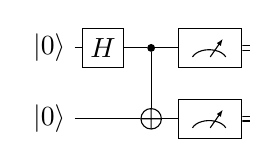
\begin{tikzpicture}[scale=1.0]
   \begin{yquant*}[register/minimum height=0.8cm]
   qubit {$\ket0$} x;
   qubit {$\ket0$} y;
   box {$H$} x;
   cnot y | x;
   measure x;
   measure y;
  \end{yquant*}
\end{tikzpicture}
\caption{\label{fig:bell}Bell circuit}
\end{subfigure}
\qquad\qquad
\begin{subfigure}[b]{.25\textwidth}
    \centering
    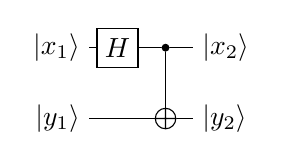
\begin{tikzpicture}[scale=1.0]
   \begin{yquant*}[register/minimum height=0.8cm]
   qubit {$\ket{x_1}$} x;
   qubit {$\ket{y_1}$} y;
   box {$H$} x;
   cnot y | x;
   output {$\ket{x_2}$} x;
   output {$\ket{y_2}$} y;
  \end{yquant*}
\end{tikzpicture}
\caption{\label{fig:bellqcore}Quantum core}
\end{subfigure}
\qquad\qquad
\begin{subfigure}[b]{.25\textwidth}
    \centering
    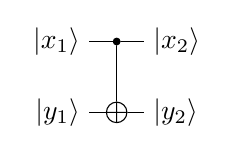
\begin{tikzpicture}[scale=1.0]
   \begin{yquant*}[register/minimum height=0.8cm]
   qubit {$\ket{x_1}$} x;
   qubit {$\ket{y_1}$} y;
   cnot y | x;
   output {$\ket{x_2}$} x;
   output {$\ket{y_2}$} y;
  \end{yquant*}
\end{tikzpicture}
\caption{\label{fig:bellccore}Classical core}
\end{subfigure}
\caption{\label{fig:bellall}A conventional quantum circuit with
  initial conditions and measurement (a); its quantum core without
  measurement and with unspecified initial and final conditions (b); and
  its classical core without explicit quantum superpositions (c).}
\end{figure}

The main ideas underlying our contributions can be illustrated with
the aid of the small examples in Fig.~\ref{fig:bellall}. In the
conventional computational mode (Fig.~\ref{fig:bell}), the execution
starts with the initial state $\ket{00}$. The first gate (Hadamard)
evolves the state to $1/\sqrt{2}(\ket{00} + \ket{10})$ which is
transformed by the controlled-not (\cx) gate to $1/\sqrt{2}(\ket{00} +
\ket{11})$. The measurements at the end produce 00 or 11 with equal
probability. Fig.~\ref{fig:bellqcore} keeps the quantum core of the
circuit, removing the measurements, and naming the inputs and outputs
with symbolic variables. Now, instead of setting $x_1=y_1=0$ and
computing forward as before, we can, for example, set $x_2=1$ and
$y_2=0$ and calculate backwards as follows: $\ket{10}$ evolves in the
backwards direction to $\ket{11}$ and then to
$1/\sqrt{2}(\ket{01}-\ket{11})$. In other words, in order to observe
$x_2y_2=10$, the variable $x_1$ should be prepared in the
superposition $1/\sqrt{2}(\ket{0}-\ket{1})$ and $y_1$ should be
prepared in the state $\ket{1}$. More interestingly, we can partially
specify the initial and final conditions. For example, we can fix
$x_1=0$ and $x_2=1$ and ask if there are any possible values for $y_1$
and $y_2$ that would be consistent with this setting. To answer the
question, we calculate, using the techniques of symbolic partial
evaluation (Methods), as follows. The initial state is $\ket{0y_1}$
which evolves to $1/\sqrt{2}(\ket{0y_1}+\ket{1y_1})$ and then to
$1/\sqrt{2}(\ket{0y_1}+\ket{1(1 \oplus y_1)})$ where $\oplus$ is the
exclusive-or operation and $1 \oplus y_1$ is the canonical way of
negating $y_1$ in the Algebraic Normal Form (ANF) of boolean
expressions (Methods). This final state can now be reconciled with the
specified final conditions $1y_2$ revealing that the settings are
consistent provided that $y_2 = 1 \oplus y_1$. We can, in fact, go one
step further and analyze the circuit without the Hadamard gate as
shown in Fig.~\ref{fig:bellccore}. The reasoning is that the role of
Hadamard is to introduce (modulo phase) uncertainty about whether
$x_1=0$ or $x_1=1$. But, again modulo phase, the same uncertainty can
be expressed by just using the variable $x_1$. Thus, in
Fig.~\ref{fig:bellccore}, we can set $y_1=0$ and $y_2=1$ and ask about
values of $x_1$ and $x_2$ that would be consistent with this
setting. We can calculate backwards from $\ket{x_21}$ as follows. The
state evolves to $\ket{x_2(1 \oplus x_2)}$ which can be reconciled
with the initial conditions yielding the constraints $x_1=x_2$ and $1
\oplus x_2 = 0$ whose solutions are $x_1 = x_2 = 1$.

\begin{figure}[t]
  \begin{subfigure}{0.5\textwidth}
  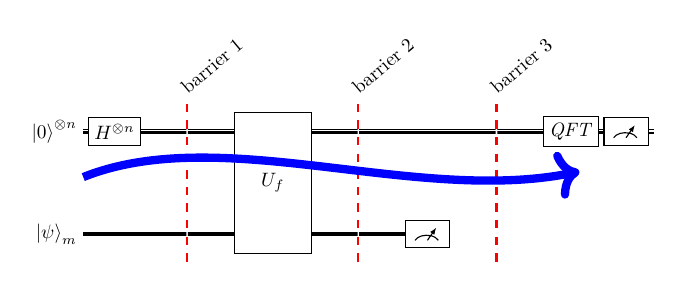
\begin{tikzpicture}[scale=0.7,every label/.style={rotate=40, anchor=south west}]
    \begin{yquant*}[operators/every barrier/.append style={red, thick},
        operator/minimum width=7mm,
        operator/separation=1mm,
        register/separation=10mm]
    qubits {$\ket0^{\otimes n}$} a;
    qubits {$\ket{\psi}_m$} b;
    box {$H^{\otimes n}$} a;
    ["barrier 1"]
    barrier (-);
    [x radius=7mm, y radius=7mm]
    box {$U_f$} (a,b);
    ["barrier 2"]
    barrier (-);
    measure b;
    discard b;
    ["barrier 3"]
    barrier (-);
    box {$\mathit{QFT}$} a;
    measure a;
    \end{yquant*}
    \draw[line width=3pt, ->, blue] (0,-1.1) .. controls (2.5,-0.1) and (6,-1.6) .. (9,-1);
  \end{tikzpicture}
  \caption{Conventional Flow}
  \end{subfigure}
  \begin{subfigure}{0.5\textwidth}
  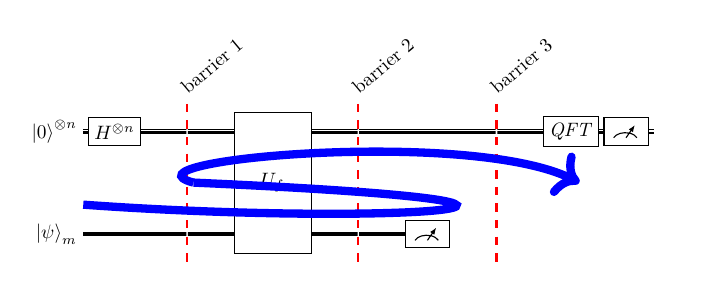
\begin{tikzpicture}[scale=0.7,every label/.style={rotate=40, anchor=south west}]
    \begin{yquant*}[operators/every barrier/.append style={red, thick},
        operator/minimum width=7mm,
        operator/separation=1mm,
        register/separation=10mm]
    qubits {$\ket0^{\otimes n}$} a;
    qubits {$\ket{\psi}_m$} b;
    box {$H^{\otimes n}$} a;
    ["barrier 1"]
    barrier (-);
    [x radius=7mm, y radius=7mm]
    box {$U_f$} (a,b);
    ["barrier 2"]
    barrier (-);
    measure b;
    discard b;
    ["barrier 3"]
    barrier (-);
    box {$\mathit{QFT}$} a;
    measure a;
  \end{yquant*}
  \draw[line width=3pt, blue] (0,-1.6) .. controls (5.5,-2) and (11,-1.6) .. (2,-1.2);
  \draw[line width=3pt, ->, blue] (2,-1.2) .. controls (0.5,-0.8) and (7,-0.2) .. (9,-1.2);
  \end{tikzpicture}
  \caption{Retrodictive Flow}
  \end{subfigure}
\caption{\label{fig:templateQC}Template quantum circuit}
\end{figure}

These insights are robust and can be implemented in software (Methods)
to analyze circuits with millions of gates for the quantum algorithms
that match the template in Fig.~\ref{fig:templateQC} (including
Deutsch, Deutsch-Jozsa, Bernstein-Vazirani, Simon, Grover, and Shor's
algorithms~\cite{doi:10.1137/S0097539796300921,deutsch,deutschJozsa,365701,doi:10.1137/S0097539795293172,nielsen_chuang_2010,10.1145/237814.237866}). The
software is completely classical, performing mixed mode executions of
the classical core of the circuits, i.e., the $U_f$ block defined as
$U_f(\ket{x}\ket{y}) = \ket{x}\ket{f(x) \oplus y}$. Specifically, in
all these algorithms, the top collection of wires (which we will call
the computational register) is prepared in a uniform superposition
which can be represented using symbolic variables. The measurement of
the bottom collection of wires (which we call the ancilla register)
after barrier 2 provides partial information about the future which
is, together with the initial conditions of the ancilla register,
sufficient to symbolically execute the circuit. In each case, instead
of the conventional execution flow depicted in
Fig.~\ref{fig:templateQC}(a), we find a possible measurement outcome
$w$ at barrier (2) and perform a symbolic retrodictive execution with
a state $\ket{xw}$ going backwards to collect the constraints on $x$
that enable us to solve the problem in question.

\subsection*{Algorithms.} 

The accompanying code includes retrodictive implementations of six
major quantum algorithms: Deutsch, Deutsch-Jozsa, Bernstein-Vazirani,
Simon, Grover, and Shor. We highlight the salient results for the
first five algorithms, and then discuss the most interesting case of
Shor's algorithm in detail.

\begin{wrapfigure}{r}{6cm}
  \centering
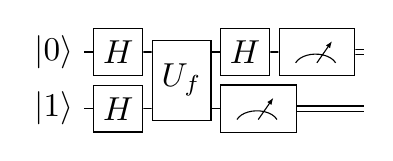
\begin{tikzpicture}[scale=1.2]
   \begin{yquant*}
   qubit {$\ket0$} x;
   qubit {$\ket1$} y;
   box {$H$} x;
   box {$H$} y;
   box {$U_f$} (x,y);
   measure y;
   box {$H$} x;
   measure x;
  \end{yquant*}
\end{tikzpicture}
\caption{\label{fig:deutsch}Quantum Circuit for the Deutsch-Jozsa
  Algorithm $(n=1)$}
\end{wrapfigure}
\paragraph*{De-Quantization.}
We abbreviate the set $\{ 0,1,\ldots,(n-1)\}$ as~$\finset{n}$. In the
Deutsch-Jozsa problem, we are given a function $\finset{2^n}
\rightarrow \finset{2}$ that is promised to be constant or balanced
and we need to distinguish the two cases. The quantum circuit
Fig.~\ref{fig:deutsch} shows the algorithm for the case $n=1$. Instead
of the conventional execution, we perform a retrodictive execution of
the $U_f$ block with an ancilla measurement~$0$, i.e., with the state
$\ket{x_{n-1}\cdots x_1x_00}$.  The result of the execution is a
symbolic formula $r$ that determines the conditions under which
$f(x_{n-1},\cdots,x_0) = 0$. When the function is constant, the
results are $0=0$ (always) or $1=0$ (never). When the function is
balanced, we get a formula that mentions the relevant variables. For
example, here are the results of three executions for balanced
functions $\finset{2^6} \rightarrow \finset{2}$:
\begin{itemize}
\item $x_0 = 0$,
\item $x_0 \oplus x_1 \oplus x_2 \oplus x_3 \oplus
    x_4 \oplus x_5 = 0$, and
\item $1 \oplus x_3x_5 \oplus x_2x_4 \oplus x_1x_5
\oplus x_0x_3 \oplus x_0x_2 \oplus x_3x_4x_5 \oplus x_2x_3x_5 \oplus
x_1x_3x_5 \oplus x_0x_3x_5 \oplus x_0x_1x_4 \oplus x_0x_1x_2 \oplus
x_2x_3x_4x_5 \oplus x_1x_3x_4x_5 \oplus x_1x_2x_4x_5 \oplus
x_1x_2x_3x_5 \oplus x_0x_3x_4x_5 \oplus x_0x_2x_4x_5 \oplus
x_0x_2x_3x_5 \oplus x_0x_1x_4x_5 \oplus x_0x_1x_3x_5 \oplus
x_0x_1x_3x_4 \oplus x_0x_1x_2x_4 \oplus x_0x_1x_2x_4x_5 \oplus
x_0x_1x_2x_3x_5 \oplus x_0x_1x_2x_3x_4 = 0$.
\end{itemize}
In the first case, the function is balanced because it produces $0$
exactly when $x_0=0$ which happens half of the time in all possible
inputs; in the second case the output of the function is the
exclusive-or of all the input variables which is another easy instance
of a balanced function. The last case is a cryptographically strong
balanced function whose output pattern is balanced but, by design,
difficult to discern~\cite{quteprints21763}.

An important insight is that we actually do not care about the exact
formula. Indeed, since we are promised that the function is either
constant or balanced, then any formula that refers to at least one
variable must indicate a balanced function. In other words, the
outcome of the algorithm can be immediately decided if the formula is
anything other than 0 or 1. Indeed, our implementation correctly
identifies all 12870 balanced functions $\finset{2^4} \rightarrow
\finset{2}$. This is significant as some of these functions produce
complicated entangled patterns during quantum evolution and could not
be de-quantized using previous approaches~\cite{djdeq}. A word of
caution though: our results assume a ``white-box'' complexity model
rather than a ``black-box'' complexity model~\cite{10.1145/3341106}.

\begin{figure}
\begin{tabular}{ll}
$u=0$ & 
  $\red{1} \oplus x_3 \oplus x_2 \oplus x_1 \oplus x_0 \oplus x_2x_3 \oplus x_1x_3 \oplus x_1x_2 \oplus x_0x_3 \oplus x_0x_2 \oplus x_0x_1 \oplus x_1x_2x_3 \oplus x_0x_2x_3$ \\
   &\quad $\oplus ~x_0x_1x_3 \oplus x_0x_1x_2 \oplus x_0x_1x_2x_3$ \\
$u=1$ & 
  $\red{x_0} \oplus x_0x_3 \oplus x_0x_2 \oplus x_0x_1 \oplus x_0x_2x_3 \oplus x_0x_1x_3 \oplus x_0x_1x_2 \oplus x_0x_1x_2x_3$ \\
$u=2$ &
  $\red{x_1} \oplus x_1x_3 \oplus x_1x_2 \oplus x_0x_1 \oplus x_1x_2x_3 \oplus x_0x_1x_3 \oplus x_0x_1x_2 \oplus x_0x_1x_2x_3$ \\
$u=3$ &
  $\red{x_0x_1} \oplus x_0x_1x_3 \oplus x_0x_1x_2 \oplus x_0x_1x_2x_3$ \\
$u=4$ &
  $\red{x_2} \oplus x_2x_3 \oplus x_1x_2 \oplus x_0x_2 \oplus x_1x_2x_3 \oplus x_0x_2x_3 \oplus x_0x_1x_2 \oplus x_0x_1x_2x_3$ \\
$u=5$ &
  $\red{x_0x_2} \oplus x_0x_2x_3 \oplus x_0x_1x_2 \oplus x_0x_1x_2x_3$ \\
$u=6$ &
  $\red{x_1x_2} \oplus x_1x_2x_3 \oplus x_0x_1x_2 \oplus x_0x_1x_2x_3$ \\
$u=7$ &
  $\red{x_0x_1x_2} \oplus x_0x_1x_2x_3$ \\
$u=8$ &
  $\red{x_3} \oplus x_2x_3 \oplus x_1x_3 \oplus x_0x_3 \oplus x_1x_2x_3 \oplus x_0x_2x_3 \oplus x_0x_1x_3 \oplus x_0x_1x_2x_3$ \\
$u=9$ &
  $\red{x_0x_3} \oplus x_0x_2x_3 \oplus x_0x_1x_3 \oplus x_0x_1x_2x_3$ \\
$u=10$ &
  $\red{x_1x_3} \oplus x_1x_2x_3 \oplus x_0x_1x_3 \oplus x_0x_1x_2x_3$ \\
$u=11$ &
  $\red{x_0x_1x_3} \oplus x_0x_1x_2x_3$ \\
$u=12$ &
  $\red{x_2x_3} \oplus x_1x_2x_3 \oplus x_0x_2x_3 \oplus x_0x_1x_2x_3$ \\
$u=13$ &
  $\red{x_0x_2x_3} \oplus x_0x_1x_2x_3$ \\
$u=14$ &
  $\red{x_1x_2x_3} \oplus x_0x_1x_2x_3$ \\
$u=15$ &
  $\red{x_0x_1x_2x_3}$
\end{tabular}
\caption{\label{fig:Grover}Result of retrodictive execution for the Grover oracle ($n=4$, $w$ in the range $\{0..15\}$). The highlighted red subformula is the binary representation of the hidden input $u$.}
\end{figure}

The discussion above suggests that the details of the equations may
not be particularly relevant for some algorithms. This would be
crucial as the satisfiability of general boolean equations is, in
general, an NP-complete
problem~\cite{4640789,Karp1972,10.1145/800157.805047}. Fortunately,
this observation does hold for other algorithms as well including the
Bernstein-Vazirani algorithm and Grover's algorithm. In both cases,
the result can be immediately read from the formula. In the
Bernstein-Vazirani case, formulae are guaranteed to be of the form
$x_1 \oplus x_3 \oplus x_4 \oplus x_5$; the secret string is then the
binary number that has a 1 at the indices of the relevant variables
$\{ 1,3,4,5 \}$. In the case for Grover, because there is a unique
input $u$ for which $f(u) = 1$, the ANF formula must include a
subformula matching the binary representation of $u$, and in fact that
subformula is guaranteed to be the shortest one as shown in
Fig.~\ref{fig:Grover}.

\begin{figure}
\[\begin{array}{l@{\quad}lllll}
\textrm{Base} & \multicolumn{4}{c}{\textrm{Equations}} & \textrm{Solution} \\[2ex]
a=11 & x_0 = 0 &&&& \red{x_0 = 0} \\
a=4,14 & 1 \oplus x_0 = 1 & x_0 = 0 &&
  & \red{x_0 = 0} \\
a=7,13 & 1 \oplus x_1 \oplus x_0x_1 = 1 & x_0x_1 = 0 & x_0 \oplus x_1 \oplus x_0x_1 = 0 &  x_0 \oplus x_0x_1 = 0 & \red{x_0=x_1=0} \\
a=2,8 & 1 \oplus x_0 \oplus x_1 \oplus x_0x_1 = 1 & x_0x_1 = 0 & x_1 \oplus x_0x_1 = 0 & x_0 \oplus x_0x_1 = 0  & \red{x_0=x_1=0}
\end{array}\]
\caption{\label{fig:shor-eqs}Equations generated by retrodictive
  execution of $a^x \mod{15}$ for different values of $a$, starting
  from observed result 1 and unknown
  $x_8x_7x_6x_5x_4x_3x_2x_1x_0$. The solution for the unknown
  variables is given in the last column.}
\end{figure}
\begin{wrapfigure}{r}{7cm}
\begin{center}
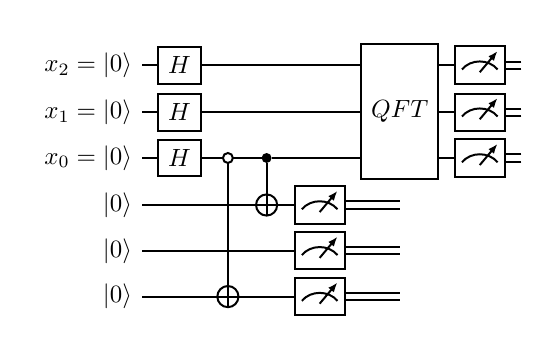
\begin{tikzpicture}
\node[scale=0.9]{    
\begin{quantikz}[row sep=0.005cm,column sep=0.22cm]
\lstick{$x_2 = \ket{0}$} & \gate{H}& \qw & \qw 
      & \qw & \gate[wires=3][0.5cm]{QFT} & \meter{} & \cw \\
\lstick{$x_1 = \ket{0}$} & \gate{H} & \qw & \qw       
      & \qw & & \meter{} & \cw \\
\lstick{$x_0 = \ket{0}$} & \gate{H} & \octrl{3} & \ctrl{1}
      & \qw & & \meter{} & \cw \\
\lstick{$\ket{0}$} & \qw & \qw & \targ{}
      & \meter{} & \cw \\
\lstick{$\ket{0}$} & \qw & \qw  & \qw
      & \meter{} & \cw \\
\lstick{$\ket{0}$} & \qw & \targ{} & \qw 
      & \meter{} & \cw
\end{quantikz}
};\end{tikzpicture}
\end{center}
\caption{\label{fig:shor15}Finding the period of $4^x \mod{15}$}
\end{wrapfigure}
\paragraph*{Shor's Algorithm}
The circuit in Fig.~\ref{fig:shor15} uses a hand-optimized
implementation of quantum oracle $U_f$ for the modular exponentiation
function $f(x) = 4^x \mod{15}$ to factor 15 using Shor's
algorithm. The white dot in the graphical representation of the first
indicates that the control is active when it is 0. In a conventional
forward execution, the state before the QFT block is:
\[
\frac{1}{2\sqrt{2}} (
  (\ket{0} + \ket{2} + \ket{4} + \ket{6}) \ket{1} + 
  (\ket{1} + \ket{3} + \ket{5} + \ket{7}) \ket{4}
  )
\]
At this point, the ancilla register is measured to either $\ket{1}$ or
$\ket{4}$. In either case, the computational register snaps to a state
of the form $\sum_{r=0}^3 \ket{a+2r}$ whose QFT has peaks at $\ket{0}$
or $\ket{4}$ making them the most likely outcomes of measurements of
the computational register. If we measure $\ket{0}$, we repeat the
experiment; otherwise we infer that the period is~2.

In the retrodictive execution, we can start with the state
$\ket{x_2x_1x_0001}$ since 1 is guaranteed to be a possible ancilla
measurement (corresponding to $f(0)$). The first \cx-gate changes the
state to $\ket{x_2x_1x_0x_001}$ and the second \cx-gate produces
$\ket{x_2x_1x_0x_00x_0}$. At that point, we reconcile the retrodictive
result of the ancilla register $\ket{x_00x_0}$ with the initial
condition $\ket{000}$ to conclude that $x_0=0$. In other words, in
order to observe the ancilla at $001$, the computational register must
be initialized to a superposition of the form $\ket{??0}$ where the
least significant bit must be 0 and the other two bits are
unconstrained. Expanding the possibilities, the first register needs
to be in a superposition of the states $\ket{000}, \ket{010},
\ket{100}$ or $\ket{110}$ and we have just inferred using purely
classical but retrodictive reasoning that the period is
2.

This result does not, in fact, require the small optimized circuit of
Fig.~\ref{fig:shor15}. In our implementation, modular exponentiation
circuits are constructed from first principles using adders and
multipliers~\cite{PhysRevA.54.147}. In the case of $f(x) = 4^x
\mod{15}$, although the unoptimized constructed circuit has 56,538
generalized Toffoli gates (controlled$^{n}$-not gates for all $n$),
the execution results in just two simple equations: $x_0 = 0$ and $1
\oplus x_0 = 1$. Furthermore, as shown in Fig.~\ref{fig:shor-eqs}, the
shape and size of the equations is largely insensitive to the choice
of 4 as the base of the exponent, leading in all cases to the
immediate conclusion that the period is either 2 or 4. When the
solution is $x_0=0$, the period is 2, and when it is $x_0=x_1=0$, the
period is~4.

The remarkable effectiveness of retrodictive computation of the Shor
instance for factoring 15 is due to a coincidence: a period that is a
power of 2 is clearly trivial to represent in the binary number system
which, after all is expressly designed for that purpose. That
coincidence repeats itself when factoring products of the (known)
Fermat primes: 3, 5, 17, 257, and 65537, and leads to small
circuits~\cite{shorFermat}. This is confirmed with our implementation
which smoothly deals with unoptimized circuits for factoring such
products. Factoring 3*17=51 using the unoptimized circuit of 177,450
generalized Toffoli gates produces just the 4 equations: $1 \oplus x_1
= 1$, $x_0 = 0$, $x_0 \oplus x_0x_1 = 0$, and $x_1 \oplus x0x1 =
0$. Even for 3*65537=196611 whose circuit has 4,328,778 generalized
Toffoli gates, the execution produces 16 small equations that refer to
just the four variables $x_0$, $x_1$, $x_2$, and $x_3$ constraining
them to be all 0, i.e., asserting that the period is 16.

\begin{wrapfigure}{r}{7cm}
  \centering
    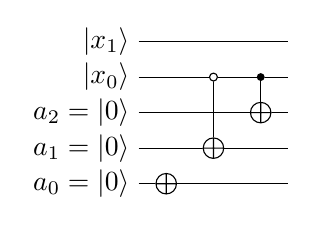
\begin{tikzpicture}[scale=1.0]
   \begin{yquant*}
   qubit {$\ket{x_1}$} x1;
   qubit {$\ket{x_0}$} x0;
   qubit {$a_2 = \ket0$} a2;
   qubit {$a_1 = \ket0$} a1;
   qubit {$a_0 = \ket0$} a0;
   not a0;
   align -;
   cnot a1 | ~x0; 
   cnot a2 | x0; 
  \end{yquant*}
\end{tikzpicture}
\caption{\label{fig:shor21}Finding the period of $4^x \mod{21}$ using
  qutrits. The three gates are from left to right are the $X$,
  $\textrm{SUM}$, and $C(X)$ gates for ternary
  arithmetic~\cite{10.5555/3179473.3179481}. The $X$ gate adds 1
  modulo 3; the controlled version $C(X)$ only increments when the
  control is equal to 2, and the \textrm{SUM} gates maps $\ket{a,b}$
  to $\ket{a,a+b}$.}
\end{wrapfigure}
Since periods that are powers of 2 are rare and special, we turn our
attention to factoring problems with other periods. The simplest such
problem is that of factoring 21 with an underlying function $f(x) =
4^x \mod{21}$ of period 3. The unoptimized circuit constructed from
the first principles has 78,600 generalized Toffoli gates; its
execution generates just three equations. But even in this rather
trivial situation, the equations span 5 pages of text!  (Supplementary
Material). A small optimization reducing the number of qubits results
in a circuit of 15,624 generalized Toffoli gates whose execution
produces still quite large, but more reasonable, equations
(Supplementary Material). To understand the reason for these unwieldy
equations, we examine a general ANF formula of the form $ X_1 \oplus
X_2 \oplus X_3 \oplus \ldots = 0$ where each $X_i$ is a conjunction of
some boolean variables, i.e., the variables in each $X$ exhibit
constructive interference as they must all be true to enable that
$X=1$. Since the entire formula must equal to 0, every $X_i = 1$ must
be offset by another $X_j = 1$, thus exhibiting negative interference
among $X_i$ and $X_j$. Generally speaking, arbitrary interference
patterns can be encoded in the formulae at the cost of making the size
of the formulae exponential in the number of variables. This
exponential blowup is actually a necessary condition for any quantum
algorithm that can offer an exponential speed-up over classical
computation~\cite{10.2307/3560059}.

It would however be incorrect to conclude that factoring 21 is
inherently harder than factoring 15. The issue is simply that the
binary number system is well-tuned to expressing patterns over powers
of 2 but a very poor match for expressing patterns over powers of
3. Indeed, we show that by just using qutrits, the circuit and
equations for factoring 21 become trivial while those for factoring 15
become unwieldy. The manually optimized circuit in
Fig.~\ref{fig:shor21} consists of just three gates; its retrodictive
execution produces two equations: $x_0=0$ and $x_0 \neq 2$, setting
$x_0=0$ and leaving $x_1$ unconstrained. The matching values in the
qutrit system as 00, 10, 20 or in decimal 0, 3, 6 clearly identifying
the period to be 3. The idea of adapting the computation to simplify
the circuit and equations is inspired by the fact that entanglement is
relative to a particular tensor product decomposition (Methods).

\printbibliography[heading=subbibliography]
\end{refsection}

%%%%%%%%%%%%%%%%%%%%%%%%%%%%%%%%%%%%%%%%%%%%%%%%%%%%%%%%%%%%%%%%%%%%%%%%%%%%%%%%%%%%%%%%%%

\newpage

\begin{refsection}
\section*{Methods}

\paragraph*{Lazy Evaluation.}
Consider a program that searches for three different numbers $x$, $y$,
and $z$ each in the range $[1..n]$ and that sum to $s$. A
well-established design principle for solving such problems is the
\emph{generate-and-test} computational paradigm. Following this
principle, a simple program to solve this problem in the programming
language Haskell is:

\begin{minted}{haskell}
generate :: Int -> [(Int,Int,Int)]
generate n =  [(x,y,z) | x <- [1..n], y <- [1..n], z <- [1..n]]

test :: Int -> [(Int,Int,Int)] -> [(Int,Int,Int)]
test s nums = [(x,y,z) | (x,y,z) <- nums, x /= y, x /= z, y /= z, x+y+z == s]

find :: Int -> Int -> (Int,Int,Int)
find s =  head . test s . generate
\end{minted}

\noindent The program consists of three functions: \verb|generate| that produces
all triples \verb|(x,y,z)| from \verb|(1,1,1)| to \verb|(n,n,n)|;
\verb|test| that checks that the numbers are different and that their
sum is equal to \verb|s|; and \verb|find| that composes the two
functions: generating all triples, testing the ones that satisfy the
condition, and returning the first solution. Running this program to
find numbers in the range $[1..6]$ that sum to 15 immediately produces
$(4,5,6)$ as expected.

But what if the range of interest was $[1..10000000]$ ? A na\"\i ve
execution of the generate-and-test method would be prohibitively
expensive as it would spend all its time generating an enormous number
of triples that are un-needed. Lazy demand-driven evaluation as
implemented in Haskell succeeds in a few seconds with the result
$(1,2,12)$, however. The idea is simple: instead of eagerly generating
all the triples, generate a process that, when queried, produces one
triple at a time on demand. Conceptually the execution starts from the
observer site which is asking for the first element of a list; this
demand is propagated to the function \verb|test| which itself
propagates the demand to the function \verb|generate|. As each triple
is generated, it is tested until one triple passes the test. This
triple is immediately returned without having to generate any
additional values.

\paragraph*{Symbolic Execution of Classical Programs.}
A well-established technique to simultaneously explore multiple paths
that a classical program could take under different inputs is
\emph{symbolic
  execution}~\cite{10.1145/390016.808445,10.1145/360248.360252,howden,10.1145/800191.805647,10.1145/3182657}. In
this execution scheme, concrete values are replaced by symbols which are
initially unconstrained. As the execution proceeds, the symbols
interact with program constructs and this typically introduces
constraints on the possible values that the symbols represent. At the
end of the execution, these constraints can be solved to infer
properties of the program under consideration. The idea is also
applicable to quantum circuits as the following example illustrates.

\paragraph*{Partial Evaluation.}
Below is a Haskell program that computes $a^n$ by repeated squaring:
\begin{minted}{haskell}
power :: Int -> Int -> Int
power a n
  | n == 0     = 1
  | n == 1     = a
  | even n     = let r = power a (n `div` 2) in r * r 
  | otherwise  = a * power a (n-1)
\end{minted}
When both inputs are known, e.g., \verb|a = 3| and \verb|n = 5|, the
program evaluates as follows:
\begin{minted}{haskell}
   power 3 5
=  3 * power 3 4
=  3 * (let r1 = power 3 2 in r1 * r1)
=  3 * (let r1 = (let r2 = power 3 1 in r2 * r2) in r1 * r1)
=  3 * (let r1 = (let r2 = 3 in r2 * r2) in r1 * r1)
=  3 * (let r1 = 9 in r1 * r1)
=  243
\end{minted}

Partial evaluation is used when we only have partial information about
the inputs. Say we only know $n=5$. A partial evaluator then attempts
to evaluate \verb|power| with symbolic input \verb|a| and actual input
\verb|n=5|. This evaluation proceeds as follows:
\begin{minted}{haskell}
   power a 5 
=  a * power a 4 
=  a * (let r1 = power a 2 in r1 * r1)
=  a * (let r1 = (let r2 = power a 1 in r2 * r2) in r1 * r1)
=  a * (let r1 = (let r2 = a in r2 * r2) in r1 * r1)
=  a * (let r1 = a * a in r1 * r1)
=  let r1 = a * a in a * r1 * r1
\end{minted}
All of this evaluation, simplification, and specialization happens
without knowledge of \verb|a|. Just knowing \verb|n| was enough to
produce a residual program that is much simpler. 

The evolution of a quantum system is typically understood as
proceeding forwards in time --- from the present to the future. As
shown in Fig.~\ref{fig:templateQC}(a), 

Since the conventional execution starts with complete ignorance about
the future, the initial state is prepared as a superposition that
includes every possibility. In a well-designed algorithm, , by the
time the computation reaches the measurement stages, the relative
phases and probability amplitudes in that enormous superposition have
become biased towards states of interest which are projected to
produce the final answer.

\paragraph*{Algebraic Normal Form (ANF).}
\label{para:anf}

~

\todo{
circuits have generalized toffoli gates: semantics (and of controls;
xor with target); ANF uses exactly those two primitives; explain

The resulting
expressions are in algebraic normal form~\cite{TOKAREVA20151} where
$+$ denotes exclusive-or. 

instances with no 'and' easy to solve

if only x and cx then symbolic execution is efficient; no need for last batch of H

can solve problem classically

connect with Gottsman-Knill
}

\begin{wrapfigure}{r}{5cm}
\begin{center}
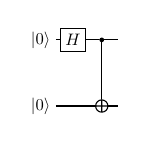
\begin{tikzpicture}[scale=0.6]
   \begin{yquant*}[register/minimum height=1.3cm]
   qubit {$\ket0$} x;
   qubit {$\ket0$} y;
   box {$H$} x;
   cnot y | x;
  \end{yquant*}
\end{tikzpicture}
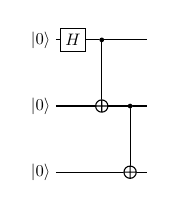
\begin{tikzpicture}[scale=0.6]
   \begin{yquant*}[register/minimum height=1.3cm]
   qubit {$\ket0$} x;
   qubit {$\ket0$} y;
   qubit {$\ket0$} z;
   box {$H$} x;
   cnot y | x;
   cnot z | y;
  \end{yquant*}
\end{tikzpicture}
\end{center}
\caption{\label{fig:bell2}Bell and GHZ States}
\end{wrapfigure}
\paragraph*{Entanglement.}
A symbolic variable represents a boolean value that can be 0 or 1;
this is similar to a qubit in a superposition $(1/\sqrt{2}) (\ket{0}
\pm \ket{1})$. Thus, it appears that $H\ket{0}$ could be represented
by a symbol~$x$ to denote the uncertainty. Surprisingly, this idea
scales to even represent maximally entangled
states. Fig.~\ref{fig:bell2}(left) shows a circuit to generate the Bell
state $(1/\sqrt{2}) (\ket{00} + \ket{11})$. By using the symbol $x$
for $H\ket{0}$, the input to the \cx-gate is $\ket{x0}$ which
evolves to $\ket{xx}$. By sharing the same symbol in two positions,
the symbolic state accurately represents the entangled Bell
state. Similarly, for the circuit in Fig.~\ref{fig:bell}(right), the
state after the Hadamard gate is $\ket{x00}$ which evolves to
$\ket{xx0}$ and then to $\ket{xxx}$ again accurately capturing the
entanglement correlations.

need for entanglement~\cite{10.2307/3560059}

\begin{wrapfigure}{r}{5cm}
\begin{center}
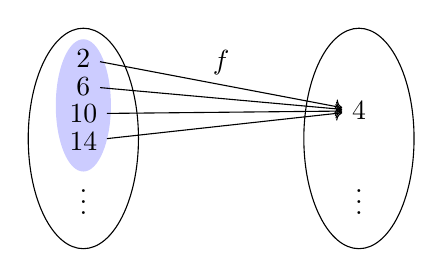
\begin{tikzpicture}[scale=0.7]
\draw (0,0) ellipse (1cm and 2cm);
\draw (5,0) circle (1cm and 2cm);
\fill[blue!20!white] (0,0.6) ellipse (0.5cm and 1.2cm);
\node (a) at (0,1.45) {2};
\node (b) at (0,0.95) {6};
\node (c) at (0,0.45) {10};
\node (d) at (0,-0.05) {14};
\node (t) at (5,0.5) {4};
\node at (0,-1) {$\vdots$};
\node at (5,-1) {$\vdots$};
\draw[->] (a) to node [above] {$f$} (t);
\draw[->] (b) -- (t);
\draw[->] (c) -- (t);
\draw[->] (d) -- (t);
\end{tikzpicture}
\end{center}
\caption{\label{fig:preimage}The pre-image of 4 under $f(x) = 7^x \mod 15$.}
\end{wrapfigure}
\paragraph*{Retrodictive Executions and Function Pre-images.}
Given finite sets $A$ and $B$, a function $f : A \rightarrow B$ and an
element $y \in B$, we define $\preim{f}{y}$, the pre-image of~$y$
under~$f$, as the set $\{ x \in A ~|~ f(x) = y \}$. For example, let
$A = B = \finset{2^4}$ and let $f(x) = 7^x \mod 15$, then the
collection of values that $f$ maps to~4, $\preim{f}{4}$, is the set
$\{ 2, 6, 10, 14 \}$ as shown in Fig.~\ref{fig:preimage}. Symbolic
retrodictive execution can be seen as a method to generate boolean
formulae that describe the pre-image of the function $f$ under
study. For the example in Fig.~\ref{fig:preimage}, retrodictive
execution might generate the formulae $x_1=1$ and $x_0=0$. The
(trivial in this case) solution for the formulae is indeed the set $\{
2, 6, 10, 14 \}$. The critical points to note, however, are that: (i)
solving the equations describing the pre-image is in general an
intractable (even for quantum computers) $\mathit{NP}$-complete
problem, and (ii) solving the equations is not needed for the quantum
algorithms in the previous section. \emph{Only some global properties
  of the pre-image are needed!} Indeed, we have already seen that for
solving the Deutsch-Jozsa problem, the only thing needed was whether
the formula contains some variables. Also for the Bernstein-Vazirani
problem, the only thing needed was the indices of the variables
occurring in the formula. For Grover's algorithm, we only need to
extract the singleton element in the pre-image and for Shor's
algorithm we only need to extract the periodicity of the elements in
the pre-image but retrodictive execution as presented so far is only
able to de-quantize some rare instances of algorithms.

To appreciate the difficulty of computing pre-images in general, note
that finding the pre-image of a function subsumes several challenging
computational problems such as pre-image attacks on hash
functions~\cite{10.1007/978-3-540-25937-4_24}, predicting
environmental conditions that allow certain reactions to take place in
computational biology~\cite{Klotz2013,akutsu2009analyses}, and finding
the pre-image of feature vectors in the space induced by a kernel in
neural networks~\cite{1353287}. More to the point, the boolean
satisfiability problem SAT is expressible as a boolean function over
the input variables and solving a SAT problem is asking for the
pre-image of \textsf{true}. Indeed, based on the conjectured existence
of one-way functions which itself implies $\mathit{P} \neq
\mathit{NP}$, all these pre-images calculations are believed to be
computationally intractable in their most general setting.

\paragraph*{Software.}

\paragraph*{Complexity Analysis.}

\paragraph*{Speculation.}

observer 1 measures wires a,b; obs2 measures wires b,c; not commuting;
each obs gives partial solution to equations; but partial solutions
cannot lead to a global solution
 
KS suggests that equations do not have unique solutions; only
materialize when you measure;

can associate a probability with each variable in a equation: look at
all solutions and see the contribution of each variable to these
solutions.

\paragraph*{Data Availability.}
All execution results will be made available and can be replicated by
executing the associated software.

\paragraph*{Code Availability.}
The computer programs used to generate the circuits and symbolically
execute the quantum algorithms retrodictively will be made publicly
available.

\paragraph*{Author Contributions.}
The idea of symbolic evaluation is due to A.S. The connection to
retrodictive quantum mechanics is due to G.O. The connection to
partial evaluation is due to J.C. Both A.S. and J.C. contributed to
the software code to run the experiments. Both A.S. and
G.O. contributed to the analysis of the quantum algorithms and their
de-quantization. All authors contributed to the writing of the
document.

\paragraph*{Competing Interests.}
No competing interests.

\paragraph*{Materials \& Correspondence.}
The corresponding author is Gerardo Ortiz. 

\paragraph*{Supplementary Information.} 
\label{par:shor21}

\paragraph*{Equations for Optimized Shor 21 Circuit.}
Equations generated by retrodictive execution of $4^x \mod{21}$
starting from observed result 1 and unknown $x$. 

$1 \oplus x_0 \oplus x_1 \oplus x_2 \oplus x_0x_2 \oplus x_0x_1x_2
\oplus x_3 \oplus x_1x_3 \oplus x_0x_1x_3 \oplus x_0x_2x_3 \oplus
x_1x_2x_3 \oplus x_4 \oplus x_0x_4 \oplus x_0x_1x_4 \oplus x_2x_4
\oplus x_1x_2x_4 \oplus x_0x_1x_2x_4 \oplus x_0x_3x_4 \oplus x_1x_3x_4
\oplus x_2x_3x_4 \oplus x_0x_2x_3x_4 \oplus x_0x_1x_2x_3x_4 \oplus x_5
\oplus x_1x_5 \oplus x_0x_1x_5 \oplus x_0x_2x_5 \oplus x_1x_2x_5
\oplus x_3x_5 \oplus x_0x_3x_5 \oplus x_0x_1x_3x_5 \oplus x_2x_3x_5
\oplus x_1x_2x_3x_5 \oplus x_0x_1x_2x_3x_5 \oplus x_0x_4x_5 \oplus
x_1x_4x_5 \oplus x_2x_4x_5 \oplus x_0x_2x_4x_5 \oplus x_0x_1x_2x_4x_5
\oplus x_3x_4x_5 \oplus x_1x_3x_4x_5 \oplus x_0x_1x_3x_4x_5 \oplus
x_0x_2x_3x_4x_5 \oplus x_1x_2x_3x_4x_5 = 1$

\bigskip

$x_1 \oplus x_0x_1 \oplus x_0x_2 \oplus x_1x_2 \oplus x_3 \oplus
x_0x_3 \oplus x_0x_1x_3 \oplus x_2x_3 \oplus x_1x_2x_3 \oplus
x_0x_1x_2x_3 \oplus x_0x_4 \oplus x_1x_4 \oplus x_2x_4 \oplus
x_0x_2x_4 \oplus x_0x_1x_2x_4 \oplus x_3x_4 \oplus x_1x_3x_4 \oplus
x_0x_1x_3x_4 \oplus x_0x_2x_3x_4 \oplus x_1x_2x_3x_4 \oplus x_5 \oplus
x_0x_5 \oplus x_0x_1x_5 \oplus x_2x_5 \oplus x_1x_2x_5 \oplus
x_0x_1x_2x_5 \oplus x_0x_3x_5 \oplus x_1x_3x_5 \oplus x_2x_3x_5 \oplus
x_0x_2x_3x_5 \oplus x_0x_1x_2x_3x_5 \oplus x_4x_5 \oplus x_1x_4x_5
\oplus x_0x_1x_4x_5 \oplus x_0x_2x_4x_5 \oplus x_1x_2x_4x_5 \oplus
x_3x_4x_5 \oplus x_0x_3x_4x_5 \oplus x_0x_1x_3x_4x_5 \oplus
x_2x_3x_4x_5 \oplus x_1x_2x_3x_4x_5 \oplus x_0x_1x_2x_3x_4x_5 = 0$

\bigskip

$x_0 \oplus x_0x_1 \oplus x_2 \oplus x_1x_2 \oplus x_0x_1x_2 \oplus
x_0x_3 \oplus x_1x_3 \oplus x_2x_3 \oplus x_0x_2x_3 \oplus
x_0x_1x_2x_3 \oplus x_4 \oplus x_1x_4 \oplus x_0x_1x_4 \oplus
x_0x_2x_4 \oplus x_1x_2x_4 \oplus x_3x_4 \oplus x_0x_3x_4 \oplus
x_0x_1x_3x_4 \oplus x_2x_3x_4 \oplus x_1x_2x_3x_4 \oplus
x_0x_1x_2x_3x_4 \oplus x_0x_5 \oplus x_1x_5 \oplus x_2x_5 \oplus
x_0x_2x_5 \oplus x_0x_1x_2x_5 \oplus x_3x_5 \oplus x_1x_3x_5 \oplus
x_0x_1x_3x_5 \oplus x_0x_2x_3x_5 \oplus x_1x_2x_3x_5 \oplus x_4x_5
\oplus x_0x_4x_5 \oplus x_0x_1x_4x_5 \oplus x_2x_4x_5 \oplus
x_1x_2x_4x_5 \oplus x_0x_1x_2x_4x_5 \oplus x_0x_3x_4x_5 \oplus
x_1x_3x_4x_5 \oplus x_2x_3x_4x_5 \oplus x_0x_2x_3x_4x_5 \oplus
x_0x_1x_2x_3x_4x_5 = 0$

\paragraph*{Equations for Unoptimized Shor 21 Circuit.}
Equations generated by retrodictive execution of $4^x \mod{21}$
starting from observed result 1 and unknown $x$. The circuit consists
of 36400 \cx-gates, 38200 \ccx-gates, and 4000 \cccx-gates. There are
only three equations but each equation is exponentially large.

$1 \oplus x0 \oplus x_1 \oplus x_2 \oplus x_0x_2 \oplus x_0x_1x_2
\oplus x_3 \oplus x_1x_3 \oplus x_0x_1x_3 \oplus x_0x_2x_3 \oplus
x_1x_2x_3 \oplus x_4 \oplus x_0x_4 \oplus x_0x_1x_4 \oplus x_2x_4
\oplus x_1x_2x_4 \oplus x_0x_1x_2x_4 \oplus x_0x_3x_4 \oplus x_1x_3x_4
\oplus x_2x_3x_4 \oplus x_0x_2x_3x_4 \oplus x_0x_1x_2x_3x_4 \oplus x_5
\oplus x_1x_5 \oplus x_0x_1x_5 \oplus x_0x_2x_5 \oplus x_1x_2x_5
\oplus x_3x_5 \oplus x_0x_3x_5 \oplus x_0x_1x_3x_5 \oplus x_2x_3x_5
\oplus x_1x_2x_3x_5 \oplus x_0x_1x_2x_3x_5 \oplus x_0x_4x_5 \oplus
x_1x_4x_5 \oplus x_2x_4x_5 \oplus x_0x_2x_4x_5 \oplus x_0x_1x_2x_4x_5
\oplus x_3x_4x_5 \oplus x_1x_3x_4x_5 \oplus x_0x_1x_3x_4x_5 \oplus
x_0x_2x_3x_4x_5 \oplus x_1x_2x_3x_4x_5 \oplus x_6 \oplus x_0x_6 \oplus
x_0x_1x_6 \oplus x_2x_6 \oplus x_1x_2x_6 \oplus x_0x_1x_2x_6 \oplus
x_0x_3x_6 \oplus x_1x_3x_6 \oplus x_2x_3x_6 \oplus x_0x_2x_3x_6 \oplus
x_0x_1x_2x_3x_6 \oplus x_4x_6 \oplus x_1x_4x_6 \oplus x_0x_1x_4x_6
\oplus x_0x_2x_4x_6 \oplus x_1x_2x_4x_6 \oplus x_3x_4x_6 \oplus
x_0x_3x_4x_6 \oplus x_0x_1x_3x_4x_6 \oplus x_2x_3x_4x_6 \oplus
x_1x_2x_3x_4x_6 \oplus x_0x_1x_2x_3x_4x_6 \oplus x_0x_5x_6 \oplus
x_1x_5x_6 \oplus x_2x_5x_6 \oplus x_0x_2x_5x_6 \oplus x_0x_1x_2x_5x_6
\oplus x_3x_5x_6 \oplus x_1x_3x_5x_6 \oplus x_0x_1x_3x_5x_6 \oplus
x_0x_2x_3x_5x_6 \oplus x_1x_2x_3x_5x_6 \oplus x_4x_5x_6 \oplus
x_0x_4x_5x_6 \oplus x_0x_1x_4x_5x_6 \oplus x_2x_4x_5x_6 \oplus
x_1x_2x_4x_5x_6 \oplus x_0x_1x_2x_4x_5x_6 \oplus x_0x_3x_4x_5x_6
\oplus x_1x_3x_4x_5x_6 \oplus x_2x_3x_4x_5x_6 \oplus
x_0x_2x_3x_4x_5x_6 \oplus x_0x_1x_2x_3x_4x_5x_6 \oplus x_7 \oplus
x_1x_7 \oplus x_0x_1x_7 \oplus x_0x_2x_7 \oplus x_1x_2x_7 \oplus
x_3x_7 \oplus x_0x_3x_7 \oplus x_0x_1x_3x_7 \oplus x_2x_3x_7 \oplus
x_1x_2x_3x_7 \oplus x_0x_1x_2x_3x_7 \oplus x_0x_4x_7 \oplus x_1x_4x_7
\oplus x_2x_4x_7 \oplus x_0x_2x_4x_7 \oplus x_0x_1x_2x_4x_7 \oplus
x_3x_4x_7 \oplus x_1x_3x_4x_7 \oplus x_0x_1x_3x_4x_7 \oplus
x_0x_2x_3x_4x_7 \oplus x_1x_2x_3x_4x_7 \oplus x_5x_7 \oplus x_0x_5x_7
\oplus x_0x_1x_5x_7 \oplus x_2x_5x_7 \oplus x_1x_2x_5x_7 \oplus
x_0x_1x_2x_5x_7 \oplus x_0x_3x_5x_7 \oplus x_1x_3x_5x_7 \oplus
x_2x_3x_5x_7 \oplus x_0x_2x_3x_5x_7 \oplus x_0x_1x_2x_3x_5x_7 \oplus
x_4x_5x_7 \oplus x_1x_4x_5x_7 \oplus x_0x_1x_4x_5x_7 \oplus
x_0x_2x_4x_5x_7 \oplus x_1x_2x_4x_5x_7 \oplus x_3x_4x_5x_7 \oplus
x_0x_3x_4x_5x_7 \oplus x_0x_1x_3x_4x_5x_7 \oplus x_2x_3x_4x_5x_7
\oplus x_1x_2x_3x_4x_5x_7 \oplus x_0x_1x_2x_3x_4x_5x_7 \oplus
x_0x_6x_7 \oplus x_1x_6x_7 \oplus x_2x_6x_7 \oplus x_0x_2x_6x_7 \oplus
x_0x_1x_2x_6x_7 \oplus x_3x_6x_7 \oplus x_1x_3x_6x_7 \oplus
x_0x_1x_3x_6x_7 \oplus x_0x_2x_3x_6x_7 \oplus x_1x_2x_3x_6x_7 \oplus
x_4x_6x_7 \oplus x_0x_4x_6x_7 \oplus x_0x_1x_4x_6x_7 \oplus
x_2x_4x_6x_7 \oplus x_1x_2x_4x_6x_7 \oplus x_0x_1x_2x_4x_6x_7 \oplus
x_0x_3x_4x_6x_7 \oplus x_1x_3x_4x_6x_7 \oplus x_2x_3x_4x_6x_7 \oplus
x_0x_2x_3x_4x_6x_7 \oplus x_0x_1x_2x_3x_4x_6x_7 \oplus x_5x_6x_7
\oplus x_1x_5x_6x_7 \oplus x_0x_1x_5x_6x_7 \oplus x_0x_2x_5x_6x_7
\oplus x_1x_2x_5x_6x_7 \oplus x_3x_5x_6x_7 \oplus x_0x_3x_5x_6x_7
\oplus x_0x_1x_3x_5x_6x_7 \oplus x_2x_3x_5x_6x_7 \oplus
x_1x_2x_3x_5x_6x_7 \oplus x_0x_1x_2x_3x_5x_6x_7 \oplus x_0x_4x_5x_6x_7
\oplus x_1x_4x_5x_6x_7 \oplus x_2x_4x_5x_6x_7 \oplus
x_0x_2x_4x_5x_6x_7 \oplus x_0x_1x_2x_4x_5x_6x_7 \oplus x_3x_4x_5x_6x_7
\oplus x_1x_3x_4x_5x_6x_7 \oplus x_0x_1x_3x_4x_5x_6x_7 \oplus
x_0x_2x_3x_4x_5x_6x_7 \oplus x_1x_2x_3x_4x_5x_6x_7 \oplus x_8 \oplus
x_0x_8 \oplus x_0x_1x_8 \oplus x_2x_8 \oplus x_1x_2x_8 \oplus
x_0x_1x_2x_8 \oplus x_0x_3x_8 \oplus x_1x_3x_8 \oplus x_2x_3x_8 \oplus
x_0x_2x_3x_8 \oplus x_0x_1x_2x_3x_8 \oplus x_4x_8 \oplus x_1x_4x_8
\oplus x_0x_1x_4x_8 \oplus x_0x_2x_4x_8 \oplus x_1x_2x_4x_8 \oplus
x_3x_4x_8 \oplus x_0x_3x_4x_8 \oplus x_0x_1x_3x_4x_8 \oplus
x_2x_3x_4x_8 \oplus x_1x_2x_3x_4x_8 \oplus x_0x_1x_2x_3x_4x_8 \oplus
x_0x_5x_8 \oplus x_1x_5x_8 \oplus x_2x_5x_8 \oplus x_0x_2x_5x_8 \oplus
x_0x_1x_2x_5x_8 \oplus x_3x_5x_8 \oplus x_1x_3x_5x_8 \oplus
x_0x_1x_3x_5x_8 \oplus x_0x_2x_3x_5x_8 \oplus x_1x_2x_3x_5x_8 \oplus
x_4x_5x_8 \oplus x_0x_4x_5x_8 \oplus x_0x_1x_4x_5x_8 \oplus
x_2x_4x_5x_8 \oplus x_1x_2x_4x_5x_8 \oplus x_0x_1x_2x_4x_5x_8 \oplus
x_0x_3x_4x_5x_8 \oplus x_1x_3x_4x_5x_8 \oplus x_2x_3x_4x_5x_8 \oplus
x_0x_2x_3x_4x_5x_8 \oplus x_0x_1x_2x_3x_4x_5x_8 \oplus x_6x_8 \oplus
x_1x_6x_8 \oplus x_0x_1x_6x_8 \oplus x_0x_2x_6x_8 \oplus x_1x_2x_6x_8
\oplus x_3x_6x_8 \oplus x_0x_3x_6x_8 \oplus x_0x_1x_3x_6x_8 \oplus
x_2x_3x_6x_8 \oplus x_1x_2x_3x_6x_8 \oplus x_0x_1x_2x_3x_6x_8 \oplus
x_0x_4x_6x_8 \oplus x_1x_4x_6x_8 \oplus x_2x_4x_6x_8 \oplus
x_0x_2x_4x_6x_8 \oplus x_0x_1x_2x_4x_6x_8 \oplus x_3x_4x_6x_8 \oplus
x_1x_3x_4x_6x_8 \oplus x_0x_1x_3x_4x_6x_8 \oplus x_0x_2x_3x_4x_6x_8
\oplus x_1x_2x_3x_4x_6x_8 \oplus x_5x_6x_8 \oplus x_0x_5x_6x_8 \oplus
x_0x_1x_5x_6x_8 \oplus x_2x_5x_6x_8 \oplus x_1x_2x_5x_6x_8 \oplus
x_0x_1x_2x_5x_6x_8 \oplus x_0x_3x_5x_6x_8 \oplus x_1x_3x_5x_6x_8
\oplus x_2x_3x_5x_6x_8 \oplus x_0x_2x_3x_5x_6x_8 \oplus
x_0x_1x_2x_3x_5x_6x_8 \oplus x_4x_5x_6x_8 \oplus x_1x_4x_5x_6x_8
\oplus x_0x_1x_4x_5x_6x_8 \oplus x_0x_2x_4x_5x_6x_8 \oplus
x_1x_2x_4x_5x_6x_8 \oplus x_3x_4x_5x_6x_8 \oplus x_0x_3x_4x_5x_6x_8
\oplus x_0x_1x_3x_4x_5x_6x_8 \oplus x_2x_3x_4x_5x_6x_8 \oplus
x_1x_2x_3x_4x_5x_6x_8 \oplus x_0x_1x_2x_3x_4x_5x_6x_8 \oplus x_0x_7x_8
\oplus x_1x_7x_8 \oplus x_2x_7x_8 \oplus x_0x_2x_7x_8 \oplus
x_0x_1x_2x_7x_8 \oplus x_3x_7x_8 \oplus x_1x_3x_7x_8 \oplus
x_0x_1x_3x_7x_8 \oplus x_0x_2x_3x_7x_8 \oplus x_1x_2x_3x_7x_8 \oplus
x_4x_7x_8 \oplus x_0x_4x_7x_8 \oplus x_0x_1x_4x_7x_8 \oplus
x_2x_4x_7x_8 \oplus x_1x_2x_4x_7x_8 \oplus x_0x_1x_2x_4x_7x_8 \oplus
x_0x_3x_4x_7x_8 \oplus x_1x_3x_4x_7x_8 \oplus x_2x_3x_4x_7x_8 \oplus
x_0x_2x_3x_4x_7x_8 \oplus x_0x_1x_2x_3x_4x_7x_8 \oplus x_5x_7x_8
\oplus x_1x_5x_7x_8 \oplus x_0x_1x_5x_7x_8 \oplus x_0x_2x_5x_7x_8
\oplus x_1x_2x_5x_7x_8 \oplus x_3x_5x_7x_8 \oplus x_0x_3x_5x_7x_8
\oplus x_0x_1x_3x_5x_7x_8 \oplus x_2x_3x_5x_7x_8 \oplus
x_1x_2x_3x_5x_7x_8 \oplus x_0x_1x_2x_3x_5x_7x_8 \oplus x_0x_4x_5x_7x_8
\oplus x_1x_4x_5x_7x_8 \oplus x_2x_4x_5x_7x_8 \oplus
x_0x_2x_4x_5x_7x_8 \oplus x_0x_1x_2x_4x_5x_7x_8 \oplus x_3x_4x_5x_7x_8
\oplus x_1x_3x_4x_5x_7x_8 \oplus x_0x_1x_3x_4x_5x_7x_8 \oplus
x_0x_2x_3x_4x_5x_7x_8 \oplus x_1x_2x_3x_4x_5x_7x_8 \oplus x_6x_7x_8
\oplus x_0x_6x_7x_8 \oplus x_0x_1x_6x_7x_8 \oplus x_2x_6x_7x_8 \oplus
x_1x_2x_6x_7x_8 \oplus x_0x_1x_2x_6x_7x_8 \oplus x_0x_3x_6x_7x_8
\oplus x_1x_3x_6x_7x_8 \oplus x_2x_3x_6x_7x_8 \oplus
x_0x_2x_3x_6x_7x_8 \oplus x_0x_1x_2x_3x_6x_7x_8 \oplus x_4x_6x_7x_8
\oplus x_1x_4x_6x_7x_8 \oplus x_0x_1x_4x_6x_7x_8 \oplus
x_0x_2x_4x_6x_7x_8 \oplus x_1x_2x_4x_6x_7x_8 \oplus x_3x_4x_6x_7x_8
\oplus x_0x_3x_4x_6x_7x_8 \oplus x_0x_1x_3x_4x_6x_7x_8 \oplus
x_2x_3x_4x_6x_7x_8 \oplus x_1x_2x_3x_4x_6x_7x_8 \oplus
x_0x_1x_2x_3x_4x_6x_7x_8 \oplus x_0x_5x_6x_7x_8 \oplus x_1x_5x_6x_7x_8
\oplus x_2x_5x_6x_7x_8 \oplus x_0x_2x_5x_6x_7x_8 \oplus
x_0x_1x_2x_5x_6x_7x_8 \oplus x_3x_5x_6x_7x_8 \oplus x_1x_3x_5x_6x_7x_8
\oplus x_0x_1x_3x_5x_6x_7x_8 \oplus x_0x_2x_3x_5x_6x_7x_8 \oplus
x_1x_2x_3x_5x_6x_7x_8 \oplus x_4x_5x_6x_7x_8 \oplus x_0x_4x_5x_6x_7x_8
\oplus x_0x_1x_4x_5x_6x_7x_8 \oplus x_2x_4x_5x_6x_7x_8 \oplus
x_1x_2x_4x_5x_6x_7x_8 \oplus x_0x_1x_2x_4x_5x_6x_7x_8 \oplus
x_0x_3x_4x_5x_6x_7x_8 \oplus x_1x_3x_4x_5x_6x_7x_8 \oplus
x_2x_3x_4x_5x_6x_7x_8 \oplus x_0x_2x_3x_4x_5x_6x_7x_8 \oplus
x_0x_1x_2x_3x_4x_5x_6x_7x_8 \oplus x_9 \oplus x_1x_9 \oplus x_0x_1x_9
\oplus x_0x_2x_9 \oplus x_1x_2x_9 \oplus x_3x_9 \oplus x_0x_3x_9
\oplus x_0x_1x_3x_9 \oplus x_2x_3x_9 \oplus x_1x_2x_3x_9 \oplus
x_0x_1x_2x_3x_9 \oplus x_0x_4x_9 \oplus x_1x_4x_9 \oplus x_2x_4x_9
\oplus x_0x_2x_4x_9 \oplus x_0x_1x_2x_4x_9 \oplus x_3x_4x_9 \oplus
x_1x_3x_4x_9 \oplus x_0x_1x_3x_4x_9 \oplus x_0x_2x_3x_4x_9 \oplus
x_1x_2x_3x_4x_9 \oplus x_5x_9 \oplus x_0x_5x_9 \oplus x_0x_1x_5x_9
\oplus x_2x_5x_9 \oplus x_1x_2x_5x_9 \oplus x_0x_1x_2x_5x_9 \oplus
x_0x_3x_5x_9 \oplus x_1x_3x_5x_9 \oplus x_2x_3x_5x_9 \oplus
x_0x_2x_3x_5x_9 \oplus x_0x_1x_2x_3x_5x_9 \oplus x_4x_5x_9 \oplus
x_1x_4x_5x_9 \oplus x_0x_1x_4x_5x_9 \oplus x_0x_2x_4x_5x_9 \oplus
x_1x_2x_4x_5x_9 \oplus x_3x_4x_5x_9 \oplus x_0x_3x_4x_5x_9 \oplus
x_0x_1x_3x_4x_5x_9 \oplus x_2x_3x_4x_5x_9 \oplus x_1x_2x_3x_4x_5x_9
\oplus x_0x_1x_2x_3x_4x_5x_9 \oplus x_0x_6x_9 \oplus x_1x_6x_9 \oplus
x_2x_6x_9 \oplus x_0x_2x_6x_9 \oplus x_0x_1x_2x_6x_9 \oplus x_3x_6x_9
\oplus x_1x_3x_6x_9 \oplus x_0x_1x_3x_6x_9 \oplus x_0x_2x_3x_6x_9
\oplus x_1x_2x_3x_6x_9 \oplus x_4x_6x_9 \oplus x_0x_4x_6x_9 \oplus
x_0x_1x_4x_6x_9 \oplus x_2x_4x_6x_9 \oplus x_1x_2x_4x_6x_9 \oplus
x_0x_1x_2x_4x_6x_9 \oplus x_0x_3x_4x_6x_9 \oplus x_1x_3x_4x_6x_9
\oplus x_2x_3x_4x_6x_9 \oplus x_0x_2x_3x_4x_6x_9 \oplus
x_0x_1x_2x_3x_4x_6x_9 \oplus x_5x_6x_9 \oplus x_1x_5x_6x_9 \oplus
x_0x_1x_5x_6x_9 \oplus x_0x_2x_5x_6x_9 \oplus x_1x_2x_5x_6x_9 \oplus
x_3x_5x_6x_9 \oplus x_0x_3x_5x_6x_9 \oplus x_0x_1x_3x_5x_6x_9 \oplus
x_2x_3x_5x_6x_9 \oplus x_1x_2x_3x_5x_6x_9 \oplus x_0x_1x_2x_3x_5x_6x_9
\oplus x_0x_4x_5x_6x_9 \oplus x_1x_4x_5x_6x_9 \oplus x_2x_4x_5x_6x_9
\oplus x_0x_2x_4x_5x_6x_9 \oplus x_0x_1x_2x_4x_5x_6x_9 \oplus
x_3x_4x_5x_6x_9 \oplus x_1x_3x_4x_5x_6x_9 \oplus x_0x_1x_3x_4x_5x_6x_9
\oplus x_0x_2x_3x_4x_5x_6x_9 \oplus x_1x_2x_3x_4x_5x_6x_9 \oplus
x_7x_9 \oplus x_0x_7x_9 \oplus x_0x_1x_7x_9 \oplus x_2x_7x_9 \oplus
x_1x_2x_7x_9 \oplus x_0x_1x_2x_7x_9 \oplus x_0x_3x_7x_9 \oplus
x_1x_3x_7x_9 \oplus x_2x_3x_7x_9 \oplus x_0x_2x_3x_7x_9 \oplus
x_0x_1x_2x_3x_7x_9 \oplus x_4x_7x_9 \oplus x_1x_4x_7x_9 \oplus
x_0x_1x_4x_7x_9 \oplus x_0x_2x_4x_7x_9 \oplus x_1x_2x_4x_7x_9 \oplus
x_3x_4x_7x_9 \oplus x_0x_3x_4x_7x_9 \oplus x_0x_1x_3x_4x_7x_9 \oplus
x_2x_3x_4x_7x_9 \oplus x_1x_2x_3x_4x_7x_9 \oplus x_0x_1x_2x_3x_4x_7x_9
\oplus x_0x_5x_7x_9 \oplus x_1x_5x_7x_9 \oplus x_2x_5x_7x_9 \oplus
x_0x_2x_5x_7x_9 \oplus x_0x_1x_2x_5x_7x_9 \oplus x_3x_5x_7x_9 \oplus
x_1x_3x_5x_7x_9 \oplus x_0x_1x_3x_5x_7x_9 \oplus x_0x_2x_3x_5x_7x_9
\oplus x_1x_2x_3x_5x_7x_9 \oplus x_4x_5x_7x_9 \oplus x_0x_4x_5x_7x_9
\oplus x_0x_1x_4x_5x_7x_9 \oplus x_2x_4x_5x_7x_9 \oplus
x_1x_2x_4x_5x_7x_9 \oplus x_0x_1x_2x_4x_5x_7x_9 \oplus
x_0x_3x_4x_5x_7x_9 \oplus x_1x_3x_4x_5x_7x_9 \oplus x_2x_3x_4x_5x_7x_9
\oplus x_0x_2x_3x_4x_5x_7x_9 \oplus x_0x_1x_2x_3x_4x_5x_7x_9 \oplus
x_6x_7x_9 \oplus x_1x_6x_7x_9 \oplus x_0x_1x_6x_7x_9 \oplus
x_0x_2x_6x_7x_9 \oplus x_1x_2x_6x_7x_9 \oplus x_3x_6x_7x_9 \oplus
x_0x_3x_6x_7x_9 \oplus x_0x_1x_3x_6x_7x_9 \oplus x_2x_3x_6x_7x_9
\oplus x_1x_2x_3x_6x_7x_9 \oplus x_0x_1x_2x_3x_6x_7x_9 \oplus
x_0x_4x_6x_7x_9 \oplus x_1x_4x_6x_7x_9 \oplus x_2x_4x_6x_7x_9 \oplus
x_0x_2x_4x_6x_7x_9 \oplus x_0x_1x_2x_4x_6x_7x_9 \oplus x_3x_4x_6x_7x_9
\oplus x_1x_3x_4x_6x_7x_9 \oplus x_0x_1x_3x_4x_6x_7x_9 \oplus
x_0x_2x_3x_4x_6x_7x_9 \oplus x_1x_2x_3x_4x_6x_7x_9 \oplus x_5x_6x_7x_9
\oplus x_0x_5x_6x_7x_9 \oplus x_0x_1x_5x_6x_7x_9 \oplus
x_2x_5x_6x_7x_9 \oplus x_1x_2x_5x_6x_7x_9 \oplus x_0x_1x_2x_5x_6x_7x_9
\oplus x_0x_3x_5x_6x_7x_9 \oplus x_1x_3x_5x_6x_7x_9 \oplus
x_2x_3x_5x_6x_7x_9 \oplus x_0x_2x_3x_5x_6x_7x_9 \oplus
x_0x_1x_2x_3x_5x_6x_7x_9 \oplus x_4x_5x_6x_7x_9 \oplus
x_1x_4x_5x_6x_7x_9 \oplus x_0x_1x_4x_5x_6x_7x_9 \oplus
x_0x_2x_4x_5x_6x_7x_9 \oplus x_1x_2x_4x_5x_6x_7x_9 \oplus
x_3x_4x_5x_6x_7x_9 \oplus x_0x_3x_4x_5x_6x_7x_9 \oplus
x_0x_1x_3x_4x_5x_6x_7x_9 \oplus x_2x_3x_4x_5x_6x_7x_9 \oplus
x_1x_2x_3x_4x_5x_6x_7x_9 \oplus x_0x_1x_2x_3x_4x_5x_6x_7x_9 \oplus
x_0x_8x_9 \oplus x_1x_8x_9 \oplus x_2x_8x_9 \oplus x_0x_2x_8x_9 \oplus
x_0x_1x_2x_8x_9 \oplus x_3x_8x_9 \oplus x_1x_3x_8x_9 \oplus
x_0x_1x_3x_8x_9 \oplus x_0x_2x_3x_8x_9 \oplus x_1x_2x_3x_8x_9 \oplus
x_4x_8x_9 \oplus x_0x_4x_8x_9 \oplus x_0x_1x_4x_8x_9 \oplus
x_2x_4x_8x_9 \oplus x_1x_2x_4x_8x_9 \oplus x_0x_1x_2x_4x_8x_9 \oplus
x_0x_3x_4x_8x_9 \oplus x_1x_3x_4x_8x_9 \oplus x_2x_3x_4x_8x_9 \oplus
x_0x_2x_3x_4x_8x_9 \oplus x_0x_1x_2x_3x_4x_8x_9 \oplus x_5x_8x_9
\oplus x_1x_5x_8x_9 \oplus x_0x_1x_5x_8x_9 \oplus x_0x_2x_5x_8x_9
\oplus x_1x_2x_5x_8x_9 \oplus x_3x_5x_8x_9 \oplus x_0x_3x_5x_8x_9
\oplus x_0x_1x_3x_5x_8x_9 \oplus x_2x_3x_5x_8x_9 \oplus
x_1x_2x_3x_5x_8x_9 \oplus x_0x_1x_2x_3x_5x_8x_9 \oplus x_0x_4x_5x_8x_9
\oplus x_1x_4x_5x_8x_9 \oplus x_2x_4x_5x_8x_9 \oplus
x_0x_2x_4x_5x_8x_9 \oplus x_0x_1x_2x_4x_5x_8x_9 \oplus x_3x_4x_5x_8x_9
\oplus x_1x_3x_4x_5x_8x_9 \oplus x_0x_1x_3x_4x_5x_8x_9 \oplus
x_0x_2x_3x_4x_5x_8x_9 \oplus x_1x_2x_3x_4x_5x_8x_9 \oplus x_6x_8x_9
\oplus x_0x_6x_8x_9 \oplus x_0x_1x_6x_8x_9 \oplus x_2x_6x_8x_9 \oplus
x_1x_2x_6x_8x_9 \oplus x_0x_1x_2x_6x_8x_9 \oplus x_0x_3x_6x_8x_9
\oplus x_1x_3x_6x_8x_9 \oplus x_2x_3x_6x_8x_9 \oplus
x_0x_2x_3x_6x_8x_9 \oplus x_0x_1x_2x_3x_6x_8x_9 \oplus x_4x_6x_8x_9
\oplus x_1x_4x_6x_8x_9 \oplus x_0x_1x_4x_6x_8x_9 \oplus
x_0x_2x_4x_6x_8x_9 \oplus x_1x_2x_4x_6x_8x_9 \oplus x_3x_4x_6x_8x_9
\oplus x_0x_3x_4x_6x_8x_9 \oplus x_0x_1x_3x_4x_6x_8x_9 \oplus
x_2x_3x_4x_6x_8x_9 \oplus x_1x_2x_3x_4x_6x_8x_9 \oplus
x_0x_1x_2x_3x_4x_6x_8x_9 \oplus x_0x_5x_6x_8x_9 \oplus x_1x_5x_6x_8x_9
\oplus x_2x_5x_6x_8x_9 \oplus x_0x_2x_5x_6x_8x_9 \oplus
x_0x_1x_2x_5x_6x_8x_9 \oplus x_3x_5x_6x_8x_9 \oplus x_1x_3x_5x_6x_8x_9
\oplus x_0x_1x_3x_5x_6x_8x_9 \oplus x_0x_2x_3x_5x_6x_8x_9 \oplus
x_1x_2x_3x_5x_6x_8x_9 \oplus x_4x_5x_6x_8x_9 \oplus x_0x_4x_5x_6x_8x_9
\oplus x_0x_1x_4x_5x_6x_8x_9 \oplus x_2x_4x_5x_6x_8x_9 \oplus
x_1x_2x_4x_5x_6x_8x_9 \oplus x_0x_1x_2x_4x_5x_6x_8x_9 \oplus
x_0x_3x_4x_5x_6x_8x_9 \oplus x_1x_3x_4x_5x_6x_8x_9 \oplus
x_2x_3x_4x_5x_6x_8x_9 \oplus x_0x_2x_3x_4x_5x_6x_8x_9 \oplus
x_0x_1x_2x_3x_4x_5x_6x_8x_9 \oplus x_7x_8x_9 \oplus x_1x_7x_8x_9
\oplus x_0x_1x_7x_8x_9 \oplus x_0x_2x_7x_8x_9 \oplus x_1x_2x_7x_8x_9
\oplus x_3x_7x_8x_9 \oplus x_0x_3x_7x_8x_9 \oplus x_0x_1x_3x_7x_8x_9
\oplus x_2x_3x_7x_8x_9 \oplus x_1x_2x_3x_7x_8x_9 \oplus
x_0x_1x_2x_3x_7x_8x_9 \oplus x_0x_4x_7x_8x_9 \oplus x_1x_4x_7x_8x_9
\oplus x_2x_4x_7x_8x_9 \oplus x_0x_2x_4x_7x_8x_9 \oplus
x_0x_1x_2x_4x_7x_8x_9 \oplus x_3x_4x_7x_8x_9 \oplus x_1x_3x_4x_7x_8x_9
\oplus x_0x_1x_3x_4x_7x_8x_9 \oplus x_0x_2x_3x_4x_7x_8x_9 \oplus
x_1x_2x_3x_4x_7x_8x_9 \oplus x_5x_7x_8x_9 \oplus x_0x_5x_7x_8x_9
\oplus x_0x_1x_5x_7x_8x_9 \oplus x_2x_5x_7x_8x_9 \oplus
x_1x_2x_5x_7x_8x_9 \oplus x_0x_1x_2x_5x_7x_8x_9 \oplus
x_0x_3x_5x_7x_8x_9 \oplus x_1x_3x_5x_7x_8x_9 \oplus x_2x_3x_5x_7x_8x_9
\oplus x_0x_2x_3x_5x_7x_8x_9 \oplus x_0x_1x_2x_3x_5x_7x_8x_9 \oplus
x_4x_5x_7x_8x_9 \oplus x_1x_4x_5x_7x_8x_9 \oplus x_0x_1x_4x_5x_7x_8x_9
\oplus x_0x_2x_4x_5x_7x_8x_9 \oplus x_1x_2x_4x_5x_7x_8x_9 \oplus
x_3x_4x_5x_7x_8x_9 \oplus x_0x_3x_4x_5x_7x_8x_9 \oplus
x_0x_1x_3x_4x_5x_7x_8x_9 \oplus x_2x_3x_4x_5x_7x_8x_9 \oplus
x_1x_2x_3x_4x_5x_7x_8x_9 \oplus x_0x_1x_2x_3x_4x_5x_7x_8x_9 \oplus
x_0x_6x_7x_8x_9 \oplus x_1x_6x_7x_8x_9 \oplus x_2x_6x_7x_8x_9 \oplus
x_0x_2x_6x_7x_8x_9 \oplus x_0x_1x_2x_6x_7x_8x_9 \oplus x_3x_6x_7x_8x_9
\oplus x_1x_3x_6x_7x_8x_9 \oplus x_0x_1x_3x_6x_7x_8x_9 \oplus
x_0x_2x_3x_6x_7x_8x_9 \oplus x_1x_2x_3x_6x_7x_8x_9 \oplus
x_4x_6x_7x_8x_9 \oplus x_0x_4x_6x_7x_8x_9 \oplus x_0x_1x_4x_6x_7x_8x_9
\oplus x_2x_4x_6x_7x_8x_9 \oplus x_1x_2x_4x_6x_7x_8x_9 \oplus
x_0x_1x_2x_4x_6x_7x_8x_9 \oplus x_0x_3x_4x_6x_7x_8x_9 \oplus
x_1x_3x_4x_6x_7x_8x_9 \oplus x_2x_3x_4x_6x_7x_8x_9 \oplus
x_0x_2x_3x_4x_6x_7x_8x_9 \oplus x_0x_1x_2x_3x_4x_6x_7x_8x_9 \oplus
x_5x_6x_7x_8x_9 \oplus x_1x_5x_6x_7x_8x_9 \oplus x_0x_1x_5x_6x_7x_8x_9
\oplus x_0x_2x_5x_6x_7x_8x_9 \oplus x_1x_2x_5x_6x_7x_8x_9 \oplus
x_3x_5x_6x_7x_8x_9 \oplus x_0x_3x_5x_6x_7x_8x_9 \oplus
x_0x_1x_3x_5x_6x_7x_8x_9 \oplus x_2x_3x_5x_6x_7x_8x_9 \oplus
x_1x_2x_3x_5x_6x_7x_8x_9 \oplus x_0x_1x_2x_3x_5x_6x_7x_8x_9 \oplus
x_0x_4x_5x_6x_7x_8x_9 \oplus x_1x_4x_5x_6x_7x_8x_9 \oplus
x_2x_4x_5x_6x_7x_8x_9 \oplus x_0x_2x_4x_5x_6x_7x_8x_9 \oplus
x_0x_1x_2x_4x_5x_6x_7x_8x_9 \oplus x_3x_4x_5x_6x_7x_8x_9 \oplus
x_1x_3x_4x_5x_6x_7x_8x_9 \oplus x_0x_1x_3x_4x_5x_6x_7x_8x_9 \oplus
x_0x_2x_3x_4x_5x_6x_7x_8x_9 \oplus x_1x_2x_3x_4x_5x_6x_7x_8x_9 = 1$

\bigskip

$x_1 \oplus x_0x_1 \oplus x_0x_2 \oplus x_1x_2 \oplus x_3 \oplus
x_0x_3 \oplus x_0x_1x_3 \oplus x_2x_3 \oplus x_1x_2x_3 \oplus
x_0x_1x_2x_3 \oplus x_0x_4 \oplus x_1x_4 \oplus x_2x_4 \oplus
x_0x_2x_4 \oplus x_0x_1x_2x_4 \oplus x_3x_4 \oplus x_1x_3x_4 \oplus
x_0x_1x_3x_4 \oplus x_0x_2x_3x_4 \oplus x_1x_2x_3x_4 \oplus x_5 \oplus
x_0x_5 \oplus x_0x_1x_5 \oplus x_2x_5 \oplus x_1x_2x_5 \oplus
x_0x_1x_2x_5 \oplus x_0x_3x_5 \oplus x_1x_3x_5 \oplus x_2x_3x_5 \oplus
x_0x_2x_3x_5 \oplus x_0x_1x_2x_3x_5 \oplus x_4x_5 \oplus x_1x_4x_5
\oplus x_0x_1x_4x_5 \oplus x_0x_2x_4x_5 \oplus x_1x_2x_4x_5 \oplus
x_3x_4x_5 \oplus x_0x_3x_4x_5 \oplus x_0x_1x_3x_4x_5 \oplus
x_2x_3x_4x_5 \oplus x_1x_2x_3x_4x_5 \oplus x_0x_1x_2x_3x_4x_5 \oplus
x_0x_6 \oplus x_1x_6 \oplus x_2x_6 \oplus x_0x_2x_6 \oplus
x_0x_1x_2x_6 \oplus x_3x_6 \oplus x_1x_3x_6 \oplus x_0x_1x_3x_6 \oplus
x_0x_2x_3x_6 \oplus x_1x_2x_3x_6 \oplus x_4x_6 \oplus x_0x_4x_6 \oplus
x_0x_1x_4x_6 \oplus x_2x_4x_6 \oplus x_1x_2x_4x_6 \oplus
x_0x_1x_2x_4x_6 \oplus x_0x_3x_4x_6 \oplus x_1x_3x_4x_6 \oplus
x_2x_3x_4x_6 \oplus x_0x_2x_3x_4x_6 \oplus x_0x_1x_2x_3x_4x_6 \oplus
x_5x_6 \oplus x_1x_5x_6 \oplus x_0x_1x_5x_6 \oplus x_0x_2x_5x_6 \oplus
x_1x_2x_5x_6 \oplus x_3x_5x_6 \oplus x_0x_3x_5x_6 \oplus
x_0x_1x_3x_5x_6 \oplus x_2x_3x_5x_6 \oplus x_1x_2x_3x_5x_6 \oplus
x_0x_1x_2x_3x_5x_6 \oplus x_0x_4x_5x_6 \oplus x_1x_4x_5x_6 \oplus
x_2x_4x_5x_6 \oplus x_0x_2x_4x_5x_6 \oplus x_0x_1x_2x_4x_5x_6 \oplus
x_3x_4x_5x_6 \oplus x_1x_3x_4x_5x_6 \oplus x_0x_1x_3x_4x_5x_6 \oplus
x_0x_2x_3x_4x_5x_6 \oplus x_1x_2x_3x_4x_5x_6 \oplus x_7 \oplus x_0x_7
\oplus x_0x_1x_7 \oplus x_2x_7 \oplus x_1x_2x_7 \oplus x_0x_1x_2x_7
\oplus x_0x_3x_7 \oplus x_1x_3x_7 \oplus x_2x_3x_7 \oplus x_0x_2x_3x_7
\oplus x_0x_1x_2x_3x_7 \oplus x_4x_7 \oplus x_1x_4x_7 \oplus
x_0x_1x_4x_7 \oplus x_0x_2x_4x_7 \oplus x_1x_2x_4x_7 \oplus x_3x_4x_7
\oplus x_0x_3x_4x_7 \oplus x_0x_1x_3x_4x_7 \oplus x_2x_3x_4x_7 \oplus
x_1x_2x_3x_4x_7 \oplus x_0x_1x_2x_3x_4x_7 \oplus x_0x_5x_7 \oplus
x_1x_5x_7 \oplus x_2x_5x_7 \oplus x_0x_2x_5x_7 \oplus x_0x_1x_2x_5x_7
\oplus x_3x_5x_7 \oplus x_1x_3x_5x_7 \oplus x_0x_1x_3x_5x_7 \oplus
x_0x_2x_3x_5x_7 \oplus x_1x_2x_3x_5x_7 \oplus x_4x_5x_7 \oplus
x_0x_4x_5x_7 \oplus x_0x_1x_4x_5x_7 \oplus x_2x_4x_5x_7 \oplus
x_1x_2x_4x_5x_7 \oplus x_0x_1x_2x_4x_5x_7 \oplus x_0x_3x_4x_5x_7
\oplus x_1x_3x_4x_5x_7 \oplus x_2x_3x_4x_5x_7 \oplus
x_0x_2x_3x_4x_5x_7 \oplus x_0x_1x_2x_3x_4x_5x_7 \oplus x_6x_7 \oplus
x_1x_6x_7 \oplus x_0x_1x_6x_7 \oplus x_0x_2x_6x_7 \oplus x_1x_2x_6x_7
\oplus x_3x_6x_7 \oplus x_0x_3x_6x_7 \oplus x_0x_1x_3x_6x_7 \oplus
x_2x_3x_6x_7 \oplus x_1x_2x_3x_6x_7 \oplus x_0x_1x_2x_3x_6x_7 \oplus
x_0x_4x_6x_7 \oplus x_1x_4x_6x_7 \oplus x_2x_4x_6x_7 \oplus
x_0x_2x_4x_6x_7 \oplus x_0x_1x_2x_4x_6x_7 \oplus x_3x_4x_6x_7 \oplus
x_1x_3x_4x_6x_7 \oplus x_0x_1x_3x_4x_6x_7 \oplus x_0x_2x_3x_4x_6x_7
\oplus x_1x_2x_3x_4x_6x_7 \oplus x_5x_6x_7 \oplus x_0x_5x_6x_7 \oplus
x_0x_1x_5x_6x_7 \oplus x_2x_5x_6x_7 \oplus x_1x_2x_5x_6x_7 \oplus
x_0x_1x_2x_5x_6x_7 \oplus x_0x_3x_5x_6x_7 \oplus x_1x_3x_5x_6x_7
\oplus x_2x_3x_5x_6x_7 \oplus x_0x_2x_3x_5x_6x_7 \oplus
x_0x_1x_2x_3x_5x_6x_7 \oplus x_4x_5x_6x_7 \oplus x_1x_4x_5x_6x_7
\oplus x_0x_1x_4x_5x_6x_7 \oplus x_0x_2x_4x_5x_6x_7 \oplus
x_1x_2x_4x_5x_6x_7 \oplus x_3x_4x_5x_6x_7 \oplus x_0x_3x_4x_5x_6x_7
\oplus x_0x_1x_3x_4x_5x_6x_7 \oplus x_2x_3x_4x_5x_6x_7 \oplus
x_1x_2x_3x_4x_5x_6x_7 \oplus x_0x_1x_2x_3x_4x_5x_6x_7 \oplus x_0x_8
\oplus x_1x_8 \oplus x_2x_8 \oplus x_0x_2x_8 \oplus x_0x_1x_2x_8
\oplus x_3x_8 \oplus x_1x_3x_8 \oplus x_0x_1x_3x_8 \oplus x_0x_2x_3x_8
\oplus x_1x_2x_3x_8 \oplus x_4x_8 \oplus x_0x_4x_8 \oplus x_0x_1x_4x_8
\oplus x_2x_4x_8 \oplus x_1x_2x_4x_8 \oplus x_0x_1x_2x_4x_8 \oplus
x_0x_3x_4x_8 \oplus x_1x_3x_4x_8 \oplus x_2x_3x_4x_8 \oplus
x_0x_2x_3x_4x_8 \oplus x_0x_1x_2x_3x_4x_8 \oplus x_5x_8 \oplus
x_1x_5x_8 \oplus x_0x_1x_5x_8 \oplus x_0x_2x_5x_8 \oplus x_1x_2x_5x_8
\oplus x_3x_5x_8 \oplus x_0x_3x_5x_8 \oplus x_0x_1x_3x_5x_8 \oplus
x_2x_3x_5x_8 \oplus x_1x_2x_3x_5x_8 \oplus x_0x_1x_2x_3x_5x_8 \oplus
x_0x_4x_5x_8 \oplus x_1x_4x_5x_8 \oplus x_2x_4x_5x_8 \oplus
x_0x_2x_4x_5x_8 \oplus x_0x_1x_2x_4x_5x_8 \oplus x_3x_4x_5x_8 \oplus
x_1x_3x_4x_5x_8 \oplus x_0x_1x_3x_4x_5x_8 \oplus x_0x_2x_3x_4x_5x_8
\oplus x_1x_2x_3x_4x_5x_8 \oplus x_6x_8 \oplus x_0x_6x_8 \oplus
x_0x_1x_6x_8 \oplus x_2x_6x_8 \oplus x_1x_2x_6x_8 \oplus
x_0x_1x_2x_6x_8 \oplus x_0x_3x_6x_8 \oplus x_1x_3x_6x_8 \oplus
x_2x_3x_6x_8 \oplus x_0x_2x_3x_6x_8 \oplus x_0x_1x_2x_3x_6x_8 \oplus
x_4x_6x_8 \oplus x_1x_4x_6x_8 \oplus x_0x_1x_4x_6x_8 \oplus
x_0x_2x_4x_6x_8 \oplus x_1x_2x_4x_6x_8 \oplus x_3x_4x_6x_8 \oplus
x_0x_3x_4x_6x_8 \oplus x_0x_1x_3x_4x_6x_8 \oplus x_2x_3x_4x_6x_8
\oplus x_1x_2x_3x_4x_6x_8 \oplus x_0x_1x_2x_3x_4x_6x_8 \oplus
x_0x_5x_6x_8 \oplus x_1x_5x_6x_8 \oplus x_2x_5x_6x_8 \oplus
x_0x_2x_5x_6x_8 \oplus x_0x_1x_2x_5x_6x_8 \oplus x_3x_5x_6x_8 \oplus
x_1x_3x_5x_6x_8 \oplus x_0x_1x_3x_5x_6x_8 \oplus x_0x_2x_3x_5x_6x_8
\oplus x_1x_2x_3x_5x_6x_8 \oplus x_4x_5x_6x_8 \oplus x_0x_4x_5x_6x_8
\oplus x_0x_1x_4x_5x_6x_8 \oplus x_2x_4x_5x_6x_8 \oplus
x_1x_2x_4x_5x_6x_8 \oplus x_0x_1x_2x_4x_5x_6x_8 \oplus
x_0x_3x_4x_5x_6x_8 \oplus x_1x_3x_4x_5x_6x_8 \oplus x_2x_3x_4x_5x_6x_8
\oplus x_0x_2x_3x_4x_5x_6x_8 \oplus x_0x_1x_2x_3x_4x_5x_6x_8 \oplus
x_7x_8 \oplus x_1x_7x_8 \oplus x_0x_1x_7x_8 \oplus x_0x_2x_7x_8 \oplus
x_1x_2x_7x_8 \oplus x_3x_7x_8 \oplus x_0x_3x_7x_8 \oplus
x_0x_1x_3x_7x_8 \oplus x_2x_3x_7x_8 \oplus x_1x_2x_3x_7x_8 \oplus
x_0x_1x_2x_3x_7x_8 \oplus x_0x_4x_7x_8 \oplus x_1x_4x_7x_8 \oplus
x_2x_4x_7x_8 \oplus x_0x_2x_4x_7x_8 \oplus x_0x_1x_2x_4x_7x_8 \oplus
x_3x_4x_7x_8 \oplus x_1x_3x_4x_7x_8 \oplus x_0x_1x_3x_4x_7x_8 \oplus
x_0x_2x_3x_4x_7x_8 \oplus x_1x_2x_3x_4x_7x_8 \oplus x_5x_7x_8 \oplus
x_0x_5x_7x_8 \oplus x_0x_1x_5x_7x_8 \oplus x_2x_5x_7x_8 \oplus
x_1x_2x_5x_7x_8 \oplus x_0x_1x_2x_5x_7x_8 \oplus x_0x_3x_5x_7x_8
\oplus x_1x_3x_5x_7x_8 \oplus x_2x_3x_5x_7x_8 \oplus
x_0x_2x_3x_5x_7x_8 \oplus x_0x_1x_2x_3x_5x_7x_8 \oplus x_4x_5x_7x_8
\oplus x_1x_4x_5x_7x_8 \oplus x_0x_1x_4x_5x_7x_8 \oplus
x_0x_2x_4x_5x_7x_8 \oplus x_1x_2x_4x_5x_7x_8 \oplus x_3x_4x_5x_7x_8
\oplus x_0x_3x_4x_5x_7x_8 \oplus x_0x_1x_3x_4x_5x_7x_8 \oplus
x_2x_3x_4x_5x_7x_8 \oplus x_1x_2x_3x_4x_5x_7x_8 \oplus
x_0x_1x_2x_3x_4x_5x_7x_8 \oplus x_0x_6x_7x_8 \oplus x_1x_6x_7x_8
\oplus x_2x_6x_7x_8 \oplus x_0x_2x_6x_7x_8 \oplus x_0x_1x_2x_6x_7x_8
\oplus x_3x_6x_7x_8 \oplus x_1x_3x_6x_7x_8 \oplus x_0x_1x_3x_6x_7x_8
\oplus x_0x_2x_3x_6x_7x_8 \oplus x_1x_2x_3x_6x_7x_8 \oplus
x_4x_6x_7x_8 \oplus x_0x_4x_6x_7x_8 \oplus x_0x_1x_4x_6x_7x_8 \oplus
x_2x_4x_6x_7x_8 \oplus x_1x_2x_4x_6x_7x_8 \oplus x_0x_1x_2x_4x_6x_7x_8
\oplus x_0x_3x_4x_6x_7x_8 \oplus x_1x_3x_4x_6x_7x_8 \oplus
x_2x_3x_4x_6x_7x_8 \oplus x_0x_2x_3x_4x_6x_7x_8 \oplus
x_0x_1x_2x_3x_4x_6x_7x_8 \oplus x_5x_6x_7x_8 \oplus x_1x_5x_6x_7x_8
\oplus x_0x_1x_5x_6x_7x_8 \oplus x_0x_2x_5x_6x_7x_8 \oplus
x_1x_2x_5x_6x_7x_8 \oplus x_3x_5x_6x_7x_8 \oplus x_0x_3x_5x_6x_7x_8
\oplus x_0x_1x_3x_5x_6x_7x_8 \oplus x_2x_3x_5x_6x_7x_8 \oplus
x_1x_2x_3x_5x_6x_7x_8 \oplus x_0x_1x_2x_3x_5x_6x_7x_8 \oplus
x_0x_4x_5x_6x_7x_8 \oplus x_1x_4x_5x_6x_7x_8 \oplus x_2x_4x_5x_6x_7x_8
\oplus x_0x_2x_4x_5x_6x_7x_8 \oplus x_0x_1x_2x_4x_5x_6x_7x_8 \oplus
x_3x_4x_5x_6x_7x_8 \oplus x_1x_3x_4x_5x_6x_7x_8 \oplus
x_0x_1x_3x_4x_5x_6x_7x_8 \oplus x_0x_2x_3x_4x_5x_6x_7x_8 \oplus
x_1x_2x_3x_4x_5x_6x_7x_8 \oplus x_9 \oplus x_0x_9 \oplus x_0x_1x_9
\oplus x_2x_9 \oplus x_1x_2x_9 \oplus x_0x_1x_2x_9 \oplus x_0x_3x_9
\oplus x_1x_3x_9 \oplus x_2x_3x_9 \oplus x_0x_2x_3x_9 \oplus
x_0x_1x_2x_3x_9 \oplus x_4x_9 \oplus x_1x_4x_9 \oplus x_0x_1x_4x_9
\oplus x_0x_2x_4x_9 \oplus x_1x_2x_4x_9 \oplus x_3x_4x_9 \oplus
x_0x_3x_4x_9 \oplus x_0x_1x_3x_4x_9 \oplus x_2x_3x_4x_9 \oplus
x_1x_2x_3x_4x_9 \oplus x_0x_1x_2x_3x_4x_9 \oplus x_0x_5x_9 \oplus
x_1x_5x_9 \oplus x_2x_5x_9 \oplus x_0x_2x_5x_9 \oplus x_0x_1x_2x_5x_9
\oplus x_3x_5x_9 \oplus x_1x_3x_5x_9 \oplus x_0x_1x_3x_5x_9 \oplus
x_0x_2x_3x_5x_9 \oplus x_1x_2x_3x_5x_9 \oplus x_4x_5x_9 \oplus
x_0x_4x_5x_9 \oplus x_0x_1x_4x_5x_9 \oplus x_2x_4x_5x_9 \oplus
x_1x_2x_4x_5x_9 \oplus x_0x_1x_2x_4x_5x_9 \oplus x_0x_3x_4x_5x_9
\oplus x_1x_3x_4x_5x_9 \oplus x_2x_3x_4x_5x_9 \oplus
x_0x_2x_3x_4x_5x_9 \oplus x_0x_1x_2x_3x_4x_5x_9 \oplus x_6x_9 \oplus
x_1x_6x_9 \oplus x_0x_1x_6x_9 \oplus x_0x_2x_6x_9 \oplus x_1x_2x_6x_9
\oplus x_3x_6x_9 \oplus x_0x_3x_6x_9 \oplus x_0x_1x_3x_6x_9 \oplus
x_2x_3x_6x_9 \oplus x_1x_2x_3x_6x_9 \oplus x_0x_1x_2x_3x_6x_9 \oplus
x_0x_4x_6x_9 \oplus x_1x_4x_6x_9 \oplus x_2x_4x_6x_9 \oplus
x_0x_2x_4x_6x_9 \oplus x_0x_1x_2x_4x_6x_9 \oplus x_3x_4x_6x_9 \oplus
x_1x_3x_4x_6x_9 \oplus x_0x_1x_3x_4x_6x_9 \oplus x_0x_2x_3x_4x_6x_9
\oplus x_1x_2x_3x_4x_6x_9 \oplus x_5x_6x_9 \oplus x_0x_5x_6x_9 \oplus
x_0x_1x_5x_6x_9 \oplus x_2x_5x_6x_9 \oplus x_1x_2x_5x_6x_9 \oplus
x_0x_1x_2x_5x_6x_9 \oplus x_0x_3x_5x_6x_9 \oplus x_1x_3x_5x_6x_9
\oplus x_2x_3x_5x_6x_9 \oplus x_0x_2x_3x_5x_6x_9 \oplus
x_0x_1x_2x_3x_5x_6x_9 \oplus x_4x_5x_6x_9 \oplus x_1x_4x_5x_6x_9
\oplus x_0x_1x_4x_5x_6x_9 \oplus x_0x_2x_4x_5x_6x_9 \oplus
x_1x_2x_4x_5x_6x_9 \oplus x_3x_4x_5x_6x_9 \oplus x_0x_3x_4x_5x_6x_9
\oplus x_0x_1x_3x_4x_5x_6x_9 \oplus x_2x_3x_4x_5x_6x_9 \oplus
x_1x_2x_3x_4x_5x_6x_9 \oplus x_0x_1x_2x_3x_4x_5x_6x_9 \oplus x_0x_7x_9
\oplus x_1x_7x_9 \oplus x_2x_7x_9 \oplus x_0x_2x_7x_9 \oplus
x_0x_1x_2x_7x_9 \oplus x_3x_7x_9 \oplus x_1x_3x_7x_9 \oplus
x_0x_1x_3x_7x_9 \oplus x_0x_2x_3x_7x_9 \oplus x_1x_2x_3x_7x_9 \oplus
x_4x_7x_9 \oplus x_0x_4x_7x_9 \oplus x_0x_1x_4x_7x_9 \oplus
x_2x_4x_7x_9 \oplus x_1x_2x_4x_7x_9 \oplus x_0x_1x_2x_4x_7x_9 \oplus
x_0x_3x_4x_7x_9 \oplus x_1x_3x_4x_7x_9 \oplus x_2x_3x_4x_7x_9 \oplus
x_0x_2x_3x_4x_7x_9 \oplus x_0x_1x_2x_3x_4x_7x_9 \oplus x_5x_7x_9
\oplus x_1x_5x_7x_9 \oplus x_0x_1x_5x_7x_9 \oplus x_0x_2x_5x_7x_9
\oplus x_1x_2x_5x_7x_9 \oplus x_3x_5x_7x_9 \oplus x_0x_3x_5x_7x_9
\oplus x_0x_1x_3x_5x_7x_9 \oplus x_2x_3x_5x_7x_9 \oplus
x_1x_2x_3x_5x_7x_9 \oplus x_0x_1x_2x_3x_5x_7x_9 \oplus x_0x_4x_5x_7x_9
\oplus x_1x_4x_5x_7x_9 \oplus x_2x_4x_5x_7x_9 \oplus
x_0x_2x_4x_5x_7x_9 \oplus x_0x_1x_2x_4x_5x_7x_9 \oplus x_3x_4x_5x_7x_9
\oplus x_1x_3x_4x_5x_7x_9 \oplus x_0x_1x_3x_4x_5x_7x_9 \oplus
x_0x_2x_3x_4x_5x_7x_9 \oplus x_1x_2x_3x_4x_5x_7x_9 \oplus x_6x_7x_9
\oplus x_0x_6x_7x_9 \oplus x_0x_1x_6x_7x_9 \oplus x_2x_6x_7x_9 \oplus
x_1x_2x_6x_7x_9 \oplus x_0x_1x_2x_6x_7x_9 \oplus x_0x_3x_6x_7x_9
\oplus x_1x_3x_6x_7x_9 \oplus x_2x_3x_6x_7x_9 \oplus
x_0x_2x_3x_6x_7x_9 \oplus x_0x_1x_2x_3x_6x_7x_9 \oplus x_4x_6x_7x_9
\oplus x_1x_4x_6x_7x_9 \oplus x_0x_1x_4x_6x_7x_9 \oplus
x_0x_2x_4x_6x_7x_9 \oplus x_1x_2x_4x_6x_7x_9 \oplus x_3x_4x_6x_7x_9
\oplus x_0x_3x_4x_6x_7x_9 \oplus x_0x_1x_3x_4x_6x_7x_9 \oplus
x_2x_3x_4x_6x_7x_9 \oplus x_1x_2x_3x_4x_6x_7x_9 \oplus
x_0x_1x_2x_3x_4x_6x_7x_9 \oplus x_0x_5x_6x_7x_9 \oplus x_1x_5x_6x_7x_9
\oplus x_2x_5x_6x_7x_9 \oplus x_0x_2x_5x_6x_7x_9 \oplus
x_0x_1x_2x_5x_6x_7x_9 \oplus x_3x_5x_6x_7x_9 \oplus x_1x_3x_5x_6x_7x_9
\oplus x_0x_1x_3x_5x_6x_7x_9 \oplus x_0x_2x_3x_5x_6x_7x_9 \oplus
x_1x_2x_3x_5x_6x_7x_9 \oplus x_4x_5x_6x_7x_9 \oplus x_0x_4x_5x_6x_7x_9
\oplus x_0x_1x_4x_5x_6x_7x_9 \oplus x_2x_4x_5x_6x_7x_9 \oplus
x_1x_2x_4x_5x_6x_7x_9 \oplus x_0x_1x_2x_4x_5x_6x_7x_9 \oplus
x_0x_3x_4x_5x_6x_7x_9 \oplus x_1x_3x_4x_5x_6x_7x_9 \oplus
x_2x_3x_4x_5x_6x_7x_9 \oplus x_0x_2x_3x_4x_5x_6x_7x_9 \oplus
x_0x_1x_2x_3x_4x_5x_6x_7x_9 \oplus x_8x_9 \oplus x_1x_8x_9 \oplus
x_0x_1x_8x_9 \oplus x_0x_2x_8x_9 \oplus x_1x_2x_8x_9 \oplus x_3x_8x_9
\oplus x_0x_3x_8x_9 \oplus x_0x_1x_3x_8x_9 \oplus x_2x_3x_8x_9 \oplus
x_1x_2x_3x_8x_9 \oplus x_0x_1x_2x_3x_8x_9 \oplus x_0x_4x_8x_9 \oplus
x_1x_4x_8x_9 \oplus x_2x_4x_8x_9 \oplus x_0x_2x_4x_8x_9 \oplus
x_0x_1x_2x_4x_8x_9 \oplus x_3x_4x_8x_9 \oplus x_1x_3x_4x_8x_9 \oplus
x_0x_1x_3x_4x_8x_9 \oplus x_0x_2x_3x_4x_8x_9 \oplus x_1x_2x_3x_4x_8x_9
\oplus x_5x_8x_9 \oplus x_0x_5x_8x_9 \oplus x_0x_1x_5x_8x_9 \oplus
x_2x_5x_8x_9 \oplus x_1x_2x_5x_8x_9 \oplus x_0x_1x_2x_5x_8x_9 \oplus
x_0x_3x_5x_8x_9 \oplus x_1x_3x_5x_8x_9 \oplus x_2x_3x_5x_8x_9 \oplus
x_0x_2x_3x_5x_8x_9 \oplus x_0x_1x_2x_3x_5x_8x_9 \oplus x_4x_5x_8x_9
\oplus x_1x_4x_5x_8x_9 \oplus x_0x_1x_4x_5x_8x_9 \oplus
x_0x_2x_4x_5x_8x_9 \oplus x_1x_2x_4x_5x_8x_9 \oplus x_3x_4x_5x_8x_9
\oplus x_0x_3x_4x_5x_8x_9 \oplus x_0x_1x_3x_4x_5x_8x_9 \oplus
x_2x_3x_4x_5x_8x_9 \oplus x_1x_2x_3x_4x_5x_8x_9 \oplus
x_0x_1x_2x_3x_4x_5x_8x_9 \oplus x_0x_6x_8x_9 \oplus x_1x_6x_8x_9
\oplus x_2x_6x_8x_9 \oplus x_0x_2x_6x_8x_9 \oplus x_0x_1x_2x_6x_8x_9
\oplus x_3x_6x_8x_9 \oplus x_1x_3x_6x_8x_9 \oplus x_0x_1x_3x_6x_8x_9
\oplus x_0x_2x_3x_6x_8x_9 \oplus x_1x_2x_3x_6x_8x_9 \oplus
x_4x_6x_8x_9 \oplus x_0x_4x_6x_8x_9 \oplus x_0x_1x_4x_6x_8x_9 \oplus
x_2x_4x_6x_8x_9 \oplus x_1x_2x_4x_6x_8x_9 \oplus x_0x_1x_2x_4x_6x_8x_9
\oplus x_0x_3x_4x_6x_8x_9 \oplus x_1x_3x_4x_6x_8x_9 \oplus
x_2x_3x_4x_6x_8x_9 \oplus x_0x_2x_3x_4x_6x_8x_9 \oplus
x_0x_1x_2x_3x_4x_6x_8x_9 \oplus x_5x_6x_8x_9 \oplus x_1x_5x_6x_8x_9
\oplus x_0x_1x_5x_6x_8x_9 \oplus x_0x_2x_5x_6x_8x_9 \oplus
x_1x_2x_5x_6x_8x_9 \oplus x_3x_5x_6x_8x_9 \oplus x_0x_3x_5x_6x_8x_9
\oplus x_0x_1x_3x_5x_6x_8x_9 \oplus x_2x_3x_5x_6x_8x_9 \oplus
x_1x_2x_3x_5x_6x_8x_9 \oplus x_0x_1x_2x_3x_5x_6x_8x_9 \oplus
x_0x_4x_5x_6x_8x_9 \oplus x_1x_4x_5x_6x_8x_9 \oplus x_2x_4x_5x_6x_8x_9
\oplus x_0x_2x_4x_5x_6x_8x_9 \oplus x_0x_1x_2x_4x_5x_6x_8x_9 \oplus
x_3x_4x_5x_6x_8x_9 \oplus x_1x_3x_4x_5x_6x_8x_9 \oplus
x_0x_1x_3x_4x_5x_6x_8x_9 \oplus x_0x_2x_3x_4x_5x_6x_8x_9 \oplus
x_1x_2x_3x_4x_5x_6x_8x_9 \oplus x_7x_8x_9 \oplus x_0x_7x_8x_9 \oplus
x_0x_1x_7x_8x_9 \oplus x_2x_7x_8x_9 \oplus x_1x_2x_7x_8x_9 \oplus
x_0x_1x_2x_7x_8x_9 \oplus x_0x_3x_7x_8x_9 \oplus x_1x_3x_7x_8x_9
\oplus x_2x_3x_7x_8x_9 \oplus x_0x_2x_3x_7x_8x_9 \oplus
x_0x_1x_2x_3x_7x_8x_9 \oplus x_4x_7x_8x_9 \oplus x_1x_4x_7x_8x_9
\oplus x_0x_1x_4x_7x_8x_9 \oplus x_0x_2x_4x_7x_8x_9 \oplus
x_1x_2x_4x_7x_8x_9 \oplus x_3x_4x_7x_8x_9 \oplus x_0x_3x_4x_7x_8x_9
\oplus x_0x_1x_3x_4x_7x_8x_9 \oplus x_2x_3x_4x_7x_8x_9 \oplus
x_1x_2x_3x_4x_7x_8x_9 \oplus x_0x_1x_2x_3x_4x_7x_8x_9 \oplus
x_0x_5x_7x_8x_9 \oplus x_1x_5x_7x_8x_9 \oplus x_2x_5x_7x_8x_9 \oplus
x_0x_2x_5x_7x_8x_9 \oplus x_0x_1x_2x_5x_7x_8x_9 \oplus x_3x_5x_7x_8x_9
\oplus x_1x_3x_5x_7x_8x_9 \oplus x_0x_1x_3x_5x_7x_8x_9 \oplus
x_0x_2x_3x_5x_7x_8x_9 \oplus x_1x_2x_3x_5x_7x_8x_9 \oplus
x_4x_5x_7x_8x_9 \oplus x_0x_4x_5x_7x_8x_9 \oplus x_0x_1x_4x_5x_7x_8x_9
\oplus x_2x_4x_5x_7x_8x_9 \oplus x_1x_2x_4x_5x_7x_8x_9 \oplus
x_0x_1x_2x_4x_5x_7x_8x_9 \oplus x_0x_3x_4x_5x_7x_8x_9 \oplus
x_1x_3x_4x_5x_7x_8x_9 \oplus x_2x_3x_4x_5x_7x_8x_9 \oplus
x_0x_2x_3x_4x_5x_7x_8x_9 \oplus x_0x_1x_2x_3x_4x_5x_7x_8x_9 \oplus
x_6x_7x_8x_9 \oplus x_1x_6x_7x_8x_9 \oplus x_0x_1x_6x_7x_8x_9 \oplus
x_0x_2x_6x_7x_8x_9 \oplus x_1x_2x_6x_7x_8x_9 \oplus x_3x_6x_7x_8x_9
\oplus x_0x_3x_6x_7x_8x_9 \oplus x_0x_1x_3x_6x_7x_8x_9 \oplus
x_2x_3x_6x_7x_8x_9 \oplus x_1x_2x_3x_6x_7x_8x_9 \oplus
x_0x_1x_2x_3x_6x_7x_8x_9 \oplus x_0x_4x_6x_7x_8x_9 \oplus
x_1x_4x_6x_7x_8x_9 \oplus x_2x_4x_6x_7x_8x_9 \oplus
x_0x_2x_4x_6x_7x_8x_9 \oplus x_0x_1x_2x_4x_6x_7x_8x_9 \oplus
x_3x_4x_6x_7x_8x_9 \oplus x_1x_3x_4x_6x_7x_8x_9 \oplus
x_0x_1x_3x_4x_6x_7x_8x_9 \oplus x_0x_2x_3x_4x_6x_7x_8x_9 \oplus
x_1x_2x_3x_4x_6x_7x_8x_9 \oplus x_5x_6x_7x_8x_9 \oplus
x_0x_5x_6x_7x_8x_9 \oplus x_0x_1x_5x_6x_7x_8x_9 \oplus
x_2x_5x_6x_7x_8x_9 \oplus x_1x_2x_5x_6x_7x_8x_9 \oplus
x_0x_1x_2x_5x_6x_7x_8x_9 \oplus x_0x_3x_5x_6x_7x_8x_9 \oplus
x_1x_3x_5x_6x_7x_8x_9 \oplus x_2x_3x_5x_6x_7x_8x_9 \oplus
x_0x_2x_3x_5x_6x_7x_8x_9 \oplus x_0x_1x_2x_3x_5x_6x_7x_8x_9 \oplus
x_4x_5x_6x_7x_8x_9 \oplus x_1x_4x_5x_6x_7x_8x_9 \oplus
x_0x_1x_4x_5x_6x_7x_8x_9 \oplus x_0x_2x_4x_5x_6x_7x_8x_9 \oplus
x_1x_2x_4x_5x_6x_7x_8x_9 \oplus x_3x_4x_5x_6x_7x_8x_9 \oplus
x_0x_3x_4x_5x_6x_7x_8x_9 \oplus x_0x_1x_3x_4x_5x_6x_7x_8x_9 \oplus
x_2x_3x_4x_5x_6x_7x_8x_9 \oplus x_1x_2x_3x_4x_5x_6x_7x_8x_9 \oplus
x_0x_1x_2x_3x_4x_5x_6x_7x_8x_9 = 0$

\bigskip

$x_0 \oplus x_0x_1 \oplus x_2 \oplus x_1x_2 \oplus x_0x_1x_2 \oplus
x_0x_3 \oplus x_1x_3 \oplus x_2x_3 \oplus x_0x_2x_3 \oplus
x_0x_1x_2x_3 \oplus x_4 \oplus x_1x_4 \oplus x_0x_1x_4 \oplus
x_0x_2x_4 \oplus x_1x_2x_4 \oplus x_3x_4 \oplus x_0x_3x_4 \oplus
x_0x_1x_3x_4 \oplus x_2x_3x_4 \oplus x_1x_2x_3x_4 \oplus
x_0x_1x_2x_3x_4 \oplus x_0x_5 \oplus x_1x_5 \oplus x_2x_5 \oplus
x_0x_2x_5 \oplus x_0x_1x_2x_5 \oplus x_3x_5 \oplus x_1x_3x_5 \oplus
x_0x_1x_3x_5 \oplus x_0x_2x_3x_5 \oplus x_1x_2x_3x_5 \oplus x_4x_5
\oplus x_0x_4x_5 \oplus x_0x_1x_4x_5 \oplus x_2x_4x_5 \oplus
x_1x_2x_4x_5 \oplus x_0x_1x_2x_4x_5 \oplus x_0x_3x_4x_5 \oplus
x_1x_3x_4x_5 \oplus x_2x_3x_4x_5 \oplus x_0x_2x_3x_4x_5 \oplus
x_0x_1x_2x_3x_4x_5 \oplus x_6 \oplus x_1x_6 \oplus x_0x_1x_6 \oplus
x_0x_2x_6 \oplus x_1x_2x_6 \oplus x_3x_6 \oplus x_0x_3x_6 \oplus
x_0x_1x_3x_6 \oplus x_2x_3x_6 \oplus x_1x_2x_3x_6 \oplus
x_0x_1x_2x_3x_6 \oplus x_0x_4x_6 \oplus x_1x_4x_6 \oplus x_2x_4x_6
\oplus x_0x_2x_4x_6 \oplus x_0x_1x_2x_4x_6 \oplus x_3x_4x_6 \oplus
x_1x_3x_4x_6 \oplus x_0x_1x_3x_4x_6 \oplus x_0x_2x_3x_4x_6 \oplus
x_1x_2x_3x_4x_6 \oplus x_5x_6 \oplus x_0x_5x_6 \oplus x_0x_1x_5x_6
\oplus x_2x_5x_6 \oplus x_1x_2x_5x_6 \oplus x_0x_1x_2x_5x_6 \oplus
x_0x_3x_5x_6 \oplus x_1x_3x_5x_6 \oplus x_2x_3x_5x_6 \oplus
x_0x_2x_3x_5x_6 \oplus x_0x_1x_2x_3x_5x_6 \oplus x_4x_5x_6 \oplus
x_1x_4x_5x_6 \oplus x_0x_1x_4x_5x_6 \oplus x_0x_2x_4x_5x_6 \oplus
x_1x_2x_4x_5x_6 \oplus x_3x_4x_5x_6 \oplus x_0x_3x_4x_5x_6 \oplus
x_0x_1x_3x_4x_5x_6 \oplus x_2x_3x_4x_5x_6 \oplus x_1x_2x_3x_4x_5x_6
\oplus x_0x_1x_2x_3x_4x_5x_6 \oplus x_0x_7 \oplus x_1x_7 \oplus x_2x_7
\oplus x_0x_2x_7 \oplus x_0x_1x_2x_7 \oplus x_3x_7 \oplus x_1x_3x_7
\oplus x_0x_1x_3x_7 \oplus x_0x_2x_3x_7 \oplus x_1x_2x_3x_7 \oplus
x_4x_7 \oplus x_0x_4x_7 \oplus x_0x_1x_4x_7 \oplus x_2x_4x_7 \oplus
x_1x_2x_4x_7 \oplus x_0x_1x_2x_4x_7 \oplus x_0x_3x_4x_7 \oplus
x_1x_3x_4x_7 \oplus x_2x_3x_4x_7 \oplus x_0x_2x_3x_4x_7 \oplus
x_0x_1x_2x_3x_4x_7 \oplus x_5x_7 \oplus x_1x_5x_7 \oplus x_0x_1x_5x_7
\oplus x_0x_2x_5x_7 \oplus x_1x_2x_5x_7 \oplus x_3x_5x_7 \oplus
x_0x_3x_5x_7 \oplus x_0x_1x_3x_5x_7 \oplus x_2x_3x_5x_7 \oplus
x_1x_2x_3x_5x_7 \oplus x_0x_1x_2x_3x_5x_7 \oplus x_0x_4x_5x_7 \oplus
x_1x_4x_5x_7 \oplus x_2x_4x_5x_7 \oplus x_0x_2x_4x_5x_7 \oplus
x_0x_1x_2x_4x_5x_7 \oplus x_3x_4x_5x_7 \oplus x_1x_3x_4x_5x_7 \oplus
x_0x_1x_3x_4x_5x_7 \oplus x_0x_2x_3x_4x_5x_7 \oplus x_1x_2x_3x_4x_5x_7
\oplus x_6x_7 \oplus x_0x_6x_7 \oplus x_0x_1x_6x_7 \oplus x_2x_6x_7
\oplus x_1x_2x_6x_7 \oplus x_0x_1x_2x_6x_7 \oplus x_0x_3x_6x_7 \oplus
x_1x_3x_6x_7 \oplus x_2x_3x_6x_7 \oplus x_0x_2x_3x_6x_7 \oplus
x_0x_1x_2x_3x_6x_7 \oplus x_4x_6x_7 \oplus x_1x_4x_6x_7 \oplus
x_0x_1x_4x_6x_7 \oplus x_0x_2x_4x_6x_7 \oplus x_1x_2x_4x_6x_7 \oplus
x_3x_4x_6x_7 \oplus x_0x_3x_4x_6x_7 \oplus x_0x_1x_3x_4x_6x_7 \oplus
x_2x_3x_4x_6x_7 \oplus x_1x_2x_3x_4x_6x_7 \oplus x_0x_1x_2x_3x_4x_6x_7
\oplus x_0x_5x_6x_7 \oplus x_1x_5x_6x_7 \oplus x_2x_5x_6x_7 \oplus
x_0x_2x_5x_6x_7 \oplus x_0x_1x_2x_5x_6x_7 \oplus x_3x_5x_6x_7 \oplus
x_1x_3x_5x_6x_7 \oplus x_0x_1x_3x_5x_6x_7 \oplus x_0x_2x_3x_5x_6x_7
\oplus x_1x_2x_3x_5x_6x_7 \oplus x_4x_5x_6x_7 \oplus x_0x_4x_5x_6x_7
\oplus x_0x_1x_4x_5x_6x_7 \oplus x_2x_4x_5x_6x_7 \oplus
x_1x_2x_4x_5x_6x_7 \oplus x_0x_1x_2x_4x_5x_6x_7 \oplus
x_0x_3x_4x_5x_6x_7 \oplus x_1x_3x_4x_5x_6x_7 \oplus x_2x_3x_4x_5x_6x_7
\oplus x_0x_2x_3x_4x_5x_6x_7 \oplus x_0x_1x_2x_3x_4x_5x_6x_7 \oplus
x_8 \oplus x_1x_8 \oplus x_0x_1x_8 \oplus x_0x_2x_8 \oplus x_1x_2x_8
\oplus x_3x_8 \oplus x_0x_3x_8 \oplus x_0x_1x_3x_8 \oplus x_2x_3x_8
\oplus x_1x_2x_3x_8 \oplus x_0x_1x_2x_3x_8 \oplus x_0x_4x_8 \oplus
x_1x_4x_8 \oplus x_2x_4x_8 \oplus x_0x_2x_4x_8 \oplus x_0x_1x_2x_4x_8
\oplus x_3x_4x_8 \oplus x_1x_3x_4x_8 \oplus x_0x_1x_3x_4x_8 \oplus
x_0x_2x_3x_4x_8 \oplus x_1x_2x_3x_4x_8 \oplus x_5x_8 \oplus x_0x_5x_8
\oplus x_0x_1x_5x_8 \oplus x_2x_5x_8 \oplus x_1x_2x_5x_8 \oplus
x_0x_1x_2x_5x_8 \oplus x_0x_3x_5x_8 \oplus x_1x_3x_5x_8 \oplus
x_2x_3x_5x_8 \oplus x_0x_2x_3x_5x_8 \oplus x_0x_1x_2x_3x_5x_8 \oplus
x_4x_5x_8 \oplus x_1x_4x_5x_8 \oplus x_0x_1x_4x_5x_8 \oplus
x_0x_2x_4x_5x_8 \oplus x_1x_2x_4x_5x_8 \oplus x_3x_4x_5x_8 \oplus
x_0x_3x_4x_5x_8 \oplus x_0x_1x_3x_4x_5x_8 \oplus x_2x_3x_4x_5x_8
\oplus x_1x_2x_3x_4x_5x_8 \oplus x_0x_1x_2x_3x_4x_5x_8 \oplus
x_0x_6x_8 \oplus x_1x_6x_8 \oplus x_2x_6x_8 \oplus x_0x_2x_6x_8 \oplus
x_0x_1x_2x_6x_8 \oplus x_3x_6x_8 \oplus x_1x_3x_6x_8 \oplus
x_0x_1x_3x_6x_8 \oplus x_0x_2x_3x_6x_8 \oplus x_1x_2x_3x_6x_8 \oplus
x_4x_6x_8 \oplus x_0x_4x_6x_8 \oplus x_0x_1x_4x_6x_8 \oplus
x_2x_4x_6x_8 \oplus x_1x_2x_4x_6x_8 \oplus x_0x_1x_2x_4x_6x_8 \oplus
x_0x_3x_4x_6x_8 \oplus x_1x_3x_4x_6x_8 \oplus x_2x_3x_4x_6x_8 \oplus
x_0x_2x_3x_4x_6x_8 \oplus x_0x_1x_2x_3x_4x_6x_8 \oplus x_5x_6x_8
\oplus x_1x_5x_6x_8 \oplus x_0x_1x_5x_6x_8 \oplus x_0x_2x_5x_6x_8
\oplus x_1x_2x_5x_6x_8 \oplus x_3x_5x_6x_8 \oplus x_0x_3x_5x_6x_8
\oplus x_0x_1x_3x_5x_6x_8 \oplus x_2x_3x_5x_6x_8 \oplus
x_1x_2x_3x_5x_6x_8 \oplus x_0x_1x_2x_3x_5x_6x_8 \oplus x_0x_4x_5x_6x_8
\oplus x_1x_4x_5x_6x_8 \oplus x_2x_4x_5x_6x_8 \oplus
x_0x_2x_4x_5x_6x_8 \oplus x_0x_1x_2x_4x_5x_6x_8 \oplus x_3x_4x_5x_6x_8
\oplus x_1x_3x_4x_5x_6x_8 \oplus x_0x_1x_3x_4x_5x_6x_8 \oplus
x_0x_2x_3x_4x_5x_6x_8 \oplus x_1x_2x_3x_4x_5x_6x_8 \oplus x_7x_8
\oplus x_0x_7x_8 \oplus x_0x_1x_7x_8 \oplus x_2x_7x_8 \oplus
x_1x_2x_7x_8 \oplus x_0x_1x_2x_7x_8 \oplus x_0x_3x_7x_8 \oplus
x_1x_3x_7x_8 \oplus x_2x_3x_7x_8 \oplus x_0x_2x_3x_7x_8 \oplus
x_0x_1x_2x_3x_7x_8 \oplus x_4x_7x_8 \oplus x_1x_4x_7x_8 \oplus
x_0x_1x_4x_7x_8 \oplus x_0x_2x_4x_7x_8 \oplus x_1x_2x_4x_7x_8 \oplus
x_3x_4x_7x_8 \oplus x_0x_3x_4x_7x_8 \oplus x_0x_1x_3x_4x_7x_8 \oplus
x_2x_3x_4x_7x_8 \oplus x_1x_2x_3x_4x_7x_8 \oplus x_0x_1x_2x_3x_4x_7x_8
\oplus x_0x_5x_7x_8 \oplus x_1x_5x_7x_8 \oplus x_2x_5x_7x_8 \oplus
x_0x_2x_5x_7x_8 \oplus x_0x_1x_2x_5x_7x_8 \oplus x_3x_5x_7x_8 \oplus
x_1x_3x_5x_7x_8 \oplus x_0x_1x_3x_5x_7x_8 \oplus x_0x_2x_3x_5x_7x_8
\oplus x_1x_2x_3x_5x_7x_8 \oplus x_4x_5x_7x_8 \oplus x_0x_4x_5x_7x_8
\oplus x_0x_1x_4x_5x_7x_8 \oplus x_2x_4x_5x_7x_8 \oplus
x_1x_2x_4x_5x_7x_8 \oplus x_0x_1x_2x_4x_5x_7x_8 \oplus
x_0x_3x_4x_5x_7x_8 \oplus x_1x_3x_4x_5x_7x_8 \oplus x_2x_3x_4x_5x_7x_8
\oplus x_0x_2x_3x_4x_5x_7x_8 \oplus x_0x_1x_2x_3x_4x_5x_7x_8 \oplus
x_6x_7x_8 \oplus x_1x_6x_7x_8 \oplus x_0x_1x_6x_7x_8 \oplus
x_0x_2x_6x_7x_8 \oplus x_1x_2x_6x_7x_8 \oplus x_3x_6x_7x_8 \oplus
x_0x_3x_6x_7x_8 \oplus x_0x_1x_3x_6x_7x_8 \oplus x_2x_3x_6x_7x_8
\oplus x_1x_2x_3x_6x_7x_8 \oplus x_0x_1x_2x_3x_6x_7x_8 \oplus
x_0x_4x_6x_7x_8 \oplus x_1x_4x_6x_7x_8 \oplus x_2x_4x_6x_7x_8 \oplus
x_0x_2x_4x_6x_7x_8 \oplus x_0x_1x_2x_4x_6x_7x_8 \oplus x_3x_4x_6x_7x_8
\oplus x_1x_3x_4x_6x_7x_8 \oplus x_0x_1x_3x_4x_6x_7x_8 \oplus
x_0x_2x_3x_4x_6x_7x_8 \oplus x_1x_2x_3x_4x_6x_7x_8 \oplus x_5x_6x_7x_8
\oplus x_0x_5x_6x_7x_8 \oplus x_0x_1x_5x_6x_7x_8 \oplus
x_2x_5x_6x_7x_8 \oplus x_1x_2x_5x_6x_7x_8 \oplus x_0x_1x_2x_5x_6x_7x_8
\oplus x_0x_3x_5x_6x_7x_8 \oplus x_1x_3x_5x_6x_7x_8 \oplus
x_2x_3x_5x_6x_7x_8 \oplus x_0x_2x_3x_5x_6x_7x_8 \oplus
x_0x_1x_2x_3x_5x_6x_7x_8 \oplus x_4x_5x_6x_7x_8 \oplus
x_1x_4x_5x_6x_7x_8 \oplus x_0x_1x_4x_5x_6x_7x_8 \oplus
x_0x_2x_4x_5x_6x_7x_8 \oplus x_1x_2x_4x_5x_6x_7x_8 \oplus
x_3x_4x_5x_6x_7x_8 \oplus x_0x_3x_4x_5x_6x_7x_8 \oplus
x_0x_1x_3x_4x_5x_6x_7x_8 \oplus x_2x_3x_4x_5x_6x_7x_8 \oplus
x_1x_2x_3x_4x_5x_6x_7x_8 \oplus x_0x_1x_2x_3x_4x_5x_6x_7x_8 \oplus
x_0x_9 \oplus x_1x_9 \oplus x_2x_9 \oplus x_0x_2x_9 \oplus
x_0x_1x_2x_9 \oplus x_3x_9 \oplus x_1x_3x_9 \oplus x_0x_1x_3x_9 \oplus
x_0x_2x_3x_9 \oplus x_1x_2x_3x_9 \oplus x_4x_9 \oplus x_0x_4x_9 \oplus
x_0x_1x_4x_9 \oplus x_2x_4x_9 \oplus x_1x_2x_4x_9 \oplus
x_0x_1x_2x_4x_9 \oplus x_0x_3x_4x_9 \oplus x_1x_3x_4x_9 \oplus
x_2x_3x_4x_9 \oplus x_0x_2x_3x_4x_9 \oplus x_0x_1x_2x_3x_4x_9 \oplus
x_5x_9 \oplus x_1x_5x_9 \oplus x_0x_1x_5x_9 \oplus x_0x_2x_5x_9 \oplus
x_1x_2x_5x_9 \oplus x_3x_5x_9 \oplus x_0x_3x_5x_9 \oplus
x_0x_1x_3x_5x_9 \oplus x_2x_3x_5x_9 \oplus x_1x_2x_3x_5x_9 \oplus
x_0x_1x_2x_3x_5x_9 \oplus x_0x_4x_5x_9 \oplus x_1x_4x_5x_9 \oplus
x_2x_4x_5x_9 \oplus x_0x_2x_4x_5x_9 \oplus x_0x_1x_2x_4x_5x_9 \oplus
x_3x_4x_5x_9 \oplus x_1x_3x_4x_5x_9 \oplus x_0x_1x_3x_4x_5x_9 \oplus
x_0x_2x_3x_4x_5x_9 \oplus x_1x_2x_3x_4x_5x_9 \oplus x_6x_9 \oplus
x_0x_6x_9 \oplus x_0x_1x_6x_9 \oplus x_2x_6x_9 \oplus x_1x_2x_6x_9
\oplus x_0x_1x_2x_6x_9 \oplus x_0x_3x_6x_9 \oplus x_1x_3x_6x_9 \oplus
x_2x_3x_6x_9 \oplus x_0x_2x_3x_6x_9 \oplus x_0x_1x_2x_3x_6x_9 \oplus
x_4x_6x_9 \oplus x_1x_4x_6x_9 \oplus x_0x_1x_4x_6x_9 \oplus
x_0x_2x_4x_6x_9 \oplus x_1x_2x_4x_6x_9 \oplus x_3x_4x_6x_9 \oplus
x_0x_3x_4x_6x_9 \oplus x_0x_1x_3x_4x_6x_9 \oplus x_2x_3x_4x_6x_9
\oplus x_1x_2x_3x_4x_6x_9 \oplus x_0x_1x_2x_3x_4x_6x_9 \oplus
x_0x_5x_6x_9 \oplus x_1x_5x_6x_9 \oplus x_2x_5x_6x_9 \oplus
x_0x_2x_5x_6x_9 \oplus x_0x_1x_2x_5x_6x_9 \oplus x_3x_5x_6x_9 \oplus
x_1x_3x_5x_6x_9 \oplus x_0x_1x_3x_5x_6x_9 \oplus x_0x_2x_3x_5x_6x_9
\oplus x_1x_2x_3x_5x_6x_9 \oplus x_4x_5x_6x_9 \oplus x_0x_4x_5x_6x_9
\oplus x_0x_1x_4x_5x_6x_9 \oplus x_2x_4x_5x_6x_9 \oplus
x_1x_2x_4x_5x_6x_9 \oplus x_0x_1x_2x_4x_5x_6x_9 \oplus
x_0x_3x_4x_5x_6x_9 \oplus x_1x_3x_4x_5x_6x_9 \oplus x_2x_3x_4x_5x_6x_9
\oplus x_0x_2x_3x_4x_5x_6x_9 \oplus x_0x_1x_2x_3x_4x_5x_6x_9 \oplus
x_7x_9 \oplus x_1x_7x_9 \oplus x_0x_1x_7x_9 \oplus x_0x_2x_7x_9 \oplus
x_1x_2x_7x_9 \oplus x_3x_7x_9 \oplus x_0x_3x_7x_9 \oplus
x_0x_1x_3x_7x_9 \oplus x_2x_3x_7x_9 \oplus x_1x_2x_3x_7x_9 \oplus
x_0x_1x_2x_3x_7x_9 \oplus x_0x_4x_7x_9 \oplus x_1x_4x_7x_9 \oplus
x_2x_4x_7x_9 \oplus x_0x_2x_4x_7x_9 \oplus x_0x_1x_2x_4x_7x_9 \oplus
x_3x_4x_7x_9 \oplus x_1x_3x_4x_7x_9 \oplus x_0x_1x_3x_4x_7x_9 \oplus
x_0x_2x_3x_4x_7x_9 \oplus x_1x_2x_3x_4x_7x_9 \oplus x_5x_7x_9 \oplus
x_0x_5x_7x_9 \oplus x_0x_1x_5x_7x_9 \oplus x_2x_5x_7x_9 \oplus
x_1x_2x_5x_7x_9 \oplus x_0x_1x_2x_5x_7x_9 \oplus x_0x_3x_5x_7x_9
\oplus x_1x_3x_5x_7x_9 \oplus x_2x_3x_5x_7x_9 \oplus
x_0x_2x_3x_5x_7x_9 \oplus x_0x_1x_2x_3x_5x_7x_9 \oplus x_4x_5x_7x_9
\oplus x_1x_4x_5x_7x_9 \oplus x_0x_1x_4x_5x_7x_9 \oplus
x_0x_2x_4x_5x_7x_9 \oplus x_1x_2x_4x_5x_7x_9 \oplus x_3x_4x_5x_7x_9
\oplus x_0x_3x_4x_5x_7x_9 \oplus x_0x_1x_3x_4x_5x_7x_9 \oplus
x_2x_3x_4x_5x_7x_9 \oplus x_1x_2x_3x_4x_5x_7x_9 \oplus
x_0x_1x_2x_3x_4x_5x_7x_9 \oplus x_0x_6x_7x_9 \oplus x_1x_6x_7x_9
\oplus x_2x_6x_7x_9 \oplus x_0x_2x_6x_7x_9 \oplus x_0x_1x_2x_6x_7x_9
\oplus x_3x_6x_7x_9 \oplus x_1x_3x_6x_7x_9 \oplus x_0x_1x_3x_6x_7x_9
\oplus x_0x_2x_3x_6x_7x_9 \oplus x_1x_2x_3x_6x_7x_9 \oplus
x_4x_6x_7x_9 \oplus x_0x_4x_6x_7x_9 \oplus x_0x_1x_4x_6x_7x_9 \oplus
x_2x_4x_6x_7x_9 \oplus x_1x_2x_4x_6x_7x_9 \oplus x_0x_1x_2x_4x_6x_7x_9
\oplus x_0x_3x_4x_6x_7x_9 \oplus x_1x_3x_4x_6x_7x_9 \oplus
x_2x_3x_4x_6x_7x_9 \oplus x_0x_2x_3x_4x_6x_7x_9 \oplus
x_0x_1x_2x_3x_4x_6x_7x_9 \oplus x_5x_6x_7x_9 \oplus x_1x_5x_6x_7x_9
\oplus x_0x_1x_5x_6x_7x_9 \oplus x_0x_2x_5x_6x_7x_9 \oplus
x_1x_2x_5x_6x_7x_9 \oplus x_3x_5x_6x_7x_9 \oplus x_0x_3x_5x_6x_7x_9
\oplus x_0x_1x_3x_5x_6x_7x_9 \oplus x_2x_3x_5x_6x_7x_9 \oplus
x_1x_2x_3x_5x_6x_7x_9 \oplus x_0x_1x_2x_3x_5x_6x_7x_9 \oplus
x_0x_4x_5x_6x_7x_9 \oplus x_1x_4x_5x_6x_7x_9 \oplus x_2x_4x_5x_6x_7x_9
\oplus x_0x_2x_4x_5x_6x_7x_9 \oplus x_0x_1x_2x_4x_5x_6x_7x_9 \oplus
x_3x_4x_5x_6x_7x_9 \oplus x_1x_3x_4x_5x_6x_7x_9 \oplus
x_0x_1x_3x_4x_5x_6x_7x_9 \oplus x_0x_2x_3x_4x_5x_6x_7x_9 \oplus
x_1x_2x_3x_4x_5x_6x_7x_9 \oplus x_8x_9 \oplus x_0x_8x_9 \oplus
x_0x_1x_8x_9 \oplus x_2x_8x_9 \oplus x_1x_2x_8x_9 \oplus
x_0x_1x_2x_8x_9 \oplus x_0x_3x_8x_9 \oplus x_1x_3x_8x_9 \oplus
x_2x_3x_8x_9 \oplus x_0x_2x_3x_8x_9 \oplus x_0x_1x_2x_3x_8x_9 \oplus
x_4x_8x_9 \oplus x_1x_4x_8x_9 \oplus x_0x_1x_4x_8x_9 \oplus
x_0x_2x_4x_8x_9 \oplus x_1x_2x_4x_8x_9 \oplus x_3x_4x_8x_9 \oplus
x_0x_3x_4x_8x_9 \oplus x_0x_1x_3x_4x_8x_9 \oplus x_2x_3x_4x_8x_9
\oplus x_1x_2x_3x_4x_8x_9 \oplus x_0x_1x_2x_3x_4x_8x_9 \oplus
x_0x_5x_8x_9 \oplus x_1x_5x_8x_9 \oplus x_2x_5x_8x_9 \oplus
x_0x_2x_5x_8x_9 \oplus x_0x_1x_2x_5x_8x_9 \oplus x_3x_5x_8x_9 \oplus
x_1x_3x_5x_8x_9 \oplus x_0x_1x_3x_5x_8x_9 \oplus x_0x_2x_3x_5x_8x_9
\oplus x_1x_2x_3x_5x_8x_9 \oplus x_4x_5x_8x_9 \oplus x_0x_4x_5x_8x_9
\oplus x_0x_1x_4x_5x_8x_9 \oplus x_2x_4x_5x_8x_9 \oplus
x_1x_2x_4x_5x_8x_9 \oplus x_0x_1x_2x_4x_5x_8x_9 \oplus
x_0x_3x_4x_5x_8x_9 \oplus x_1x_3x_4x_5x_8x_9 \oplus x_2x_3x_4x_5x_8x_9
\oplus x_0x_2x_3x_4x_5x_8x_9 \oplus x_0x_1x_2x_3x_4x_5x_8x_9 \oplus
x_6x_8x_9 \oplus x_1x_6x_8x_9 \oplus x_0x_1x_6x_8x_9 \oplus
x_0x_2x_6x_8x_9 \oplus x_1x_2x_6x_8x_9 \oplus x_3x_6x_8x_9 \oplus
x_0x_3x_6x_8x_9 \oplus x_0x_1x_3x_6x_8x_9 \oplus x_2x_3x_6x_8x_9
\oplus x_1x_2x_3x_6x_8x_9 \oplus x_0x_1x_2x_3x_6x_8x_9 \oplus
x_0x_4x_6x_8x_9 \oplus x_1x_4x_6x_8x_9 \oplus x_2x_4x_6x_8x_9 \oplus
x_0x_2x_4x_6x_8x_9 \oplus x_0x_1x_2x_4x_6x_8x_9 \oplus x_3x_4x_6x_8x_9
\oplus x_1x_3x_4x_6x_8x_9 \oplus x_0x_1x_3x_4x_6x_8x_9 \oplus
x_0x_2x_3x_4x_6x_8x_9 \oplus x_1x_2x_3x_4x_6x_8x_9 \oplus x_5x_6x_8x_9
\oplus x_0x_5x_6x_8x_9 \oplus x_0x_1x_5x_6x_8x_9 \oplus
x_2x_5x_6x_8x_9 \oplus x_1x_2x_5x_6x_8x_9 \oplus x_0x_1x_2x_5x_6x_8x_9
\oplus x_0x_3x_5x_6x_8x_9 \oplus x_1x_3x_5x_6x_8x_9 \oplus
x_2x_3x_5x_6x_8x_9 \oplus x_0x_2x_3x_5x_6x_8x_9 \oplus
x_0x_1x_2x_3x_5x_6x_8x_9 \oplus x_4x_5x_6x_8x_9 \oplus
x_1x_4x_5x_6x_8x_9 \oplus x_0x_1x_4x_5x_6x_8x_9 \oplus
x_0x_2x_4x_5x_6x_8x_9 \oplus x_1x_2x_4x_5x_6x_8x_9 \oplus
x_3x_4x_5x_6x_8x_9 \oplus x_0x_3x_4x_5x_6x_8x_9 \oplus
x_0x_1x_3x_4x_5x_6x_8x_9 \oplus x_2x_3x_4x_5x_6x_8x_9 \oplus
x_1x_2x_3x_4x_5x_6x_8x_9 \oplus x_0x_1x_2x_3x_4x_5x_6x_8x_9 \oplus
x_0x_7x_8x_9 \oplus x_1x_7x_8x_9 \oplus x_2x_7x_8x_9 \oplus
x_0x_2x_7x_8x_9 \oplus x_0x_1x_2x_7x_8x_9 \oplus x_3x_7x_8x_9 \oplus
x_1x_3x_7x_8x_9 \oplus x_0x_1x_3x_7x_8x_9 \oplus x_0x_2x_3x_7x_8x_9
\oplus x_1x_2x_3x_7x_8x_9 \oplus x_4x_7x_8x_9 \oplus x_0x_4x_7x_8x_9
\oplus x_0x_1x_4x_7x_8x_9 \oplus x_2x_4x_7x_8x_9 \oplus
x_1x_2x_4x_7x_8x_9 \oplus x_0x_1x_2x_4x_7x_8x_9 \oplus
x_0x_3x_4x_7x_8x_9 \oplus x_1x_3x_4x_7x_8x_9 \oplus x_2x_3x_4x_7x_8x_9
\oplus x_0x_2x_3x_4x_7x_8x_9 \oplus x_0x_1x_2x_3x_4x_7x_8x_9 \oplus
x_5x_7x_8x_9 \oplus x_1x_5x_7x_8x_9 \oplus x_0x_1x_5x_7x_8x_9 \oplus
x_0x_2x_5x_7x_8x_9 \oplus x_1x_2x_5x_7x_8x_9 \oplus x_3x_5x_7x_8x_9
\oplus x_0x_3x_5x_7x_8x_9 \oplus x_0x_1x_3x_5x_7x_8x_9 \oplus
x_2x_3x_5x_7x_8x_9 \oplus x_1x_2x_3x_5x_7x_8x_9 \oplus
x_0x_1x_2x_3x_5x_7x_8x_9 \oplus x_0x_4x_5x_7x_8x_9 \oplus
x_1x_4x_5x_7x_8x_9 \oplus x_2x_4x_5x_7x_8x_9 \oplus
x_0x_2x_4x_5x_7x_8x_9 \oplus x_0x_1x_2x_4x_5x_7x_8x_9 \oplus
x_3x_4x_5x_7x_8x_9 \oplus x_1x_3x_4x_5x_7x_8x_9 \oplus
x_0x_1x_3x_4x_5x_7x_8x_9 \oplus x_0x_2x_3x_4x_5x_7x_8x_9 \oplus
x_1x_2x_3x_4x_5x_7x_8x_9 \oplus x_6x_7x_8x_9 \oplus x_0x_6x_7x_8x_9
\oplus x_0x_1x_6x_7x_8x_9 \oplus x_2x_6x_7x_8x_9 \oplus
x_1x_2x_6x_7x_8x_9 \oplus x_0x_1x_2x_6x_7x_8x_9 \oplus
x_0x_3x_6x_7x_8x_9 \oplus x_1x_3x_6x_7x_8x_9 \oplus x_2x_3x_6x_7x_8x_9
\oplus x_0x_2x_3x_6x_7x_8x_9 \oplus x_0x_1x_2x_3x_6x_7x_8x_9 \oplus
x_4x_6x_7x_8x_9 \oplus x_1x_4x_6x_7x_8x_9 \oplus x_0x_1x_4x_6x_7x_8x_9
\oplus x_0x_2x_4x_6x_7x_8x_9 \oplus x_1x_2x_4x_6x_7x_8x_9 \oplus
x_3x_4x_6x_7x_8x_9 \oplus x_0x_3x_4x_6x_7x_8x_9 \oplus
x_0x_1x_3x_4x_6x_7x_8x_9 \oplus x_2x_3x_4x_6x_7x_8x_9 \oplus
x_1x_2x_3x_4x_6x_7x_8x_9 \oplus x_0x_1x_2x_3x_4x_6x_7x_8x_9 \oplus
x_0x_5x_6x_7x_8x_9 \oplus x_1x_5x_6x_7x_8x_9 \oplus x_2x_5x_6x_7x_8x_9
\oplus x_0x_2x_5x_6x_7x_8x_9 \oplus x_0x_1x_2x_5x_6x_7x_8x_9 \oplus
x_3x_5x_6x_7x_8x_9 \oplus x_1x_3x_5x_6x_7x_8x_9 \oplus
x_0x_1x_3x_5x_6x_7x_8x_9 \oplus x_0x_2x_3x_5x_6x_7x_8x_9 \oplus
x_1x_2x_3x_5x_6x_7x_8x_9 \oplus x_4x_5x_6x_7x_8x_9 \oplus
x_0x_4x_5x_6x_7x_8x_9 \oplus x_0x_1x_4x_5x_6x_7x_8x_9 \oplus
x_2x_4x_5x_6x_7x_8x_9 \oplus x_1x_2x_4x_5x_6x_7x_8x_9 \oplus
x_0x_1x_2x_4x_5x_6x_7x_8x_9 \oplus x_0x_3x_4x_5x_6x_7x_8x_9 \oplus
x_1x_3x_4x_5x_6x_7x_8x_9 \oplus x_2x_3x_4x_5x_6x_7x_8x_9 \oplus
x_0x_2x_3x_4x_5x_6x_7x_8x_9 \oplus x_0x_1x_2x_3x_4x_5x_6x_7x_8x_9 = 0$

%%%%%%%%%%%%%%%%%%%%%%%%%%%%%%%%%%%%%%%%%%%%%%%%%%%%%%%%%%%%%%%%%%%%%%%%%%%%%%%%%%%%%%%%%%

\printbibliography[heading=subbibliography]
\end{refsection}

\end{document}

%%%%%%%%%%%%%%%%%%%%%%%%%%%%%%%%%%%%%%%%%%%%%%%%%%%%%%%%%%%%%%%%%%%%%%%%%%%%%%%%%%%%%%%%%%
%%%%%%%%%%%%%%%%%%%%%%%%%%%%%%%%%%%%%%%%%%%%%%%%%%%%%%%%%%%%%%%%%%%%%%%%%%%%%%%%%%%%%%%%%%

